% ==========================
% # Métodos Laborais       #
% ==========================

\section{Métodos Laborais}

No início do mandato, ainda no planeamento do projeto foi decidida, pela Direção, a forma de trabalhar de toda a equipa do \acrshort{neeec}. Estas decisões tiveram também em conta o feedback que foi passado dos anos anteriores e aquilo que os membros da Direção sentiam enquanto membros que eram do Núcleo. Estas regras foram apresentadas aos Coordenadores Gerais que as deveriam aplicar e transmitir aos seus Colaboradores. Quando tal não acontecia, a Direção sentiu necessidade de criar uma relação mais próxima com os Colaboradores sobrepondo-se assim um pouco os CGs, o que, na nossa opinião, teve um impacto ligeiramente negativo uma vez que não permitiu criar uma relação forte de trabalho e respeito entre todos os Colaboradores e os Coordenadores das respetivas equipas.

Uma vez que a passagem de pasta feita entre o mandato 16/17 e 17/18 foi de fraca qualidade e devido a alguma inexperiência dos membros da Direção em gerir um órgão, surgiram várias ideias de mudanças na estrutura e organização do \acrshort{neeec} que, embora tenham sido essenciais para o bom funcionamento do Núcleo, criaram alguma entropia na equipa, uma vez que eram frequentemente alteradas as regras de funcionamento interno. Desta forma, sugerimos aos próximos mandatos a criação, logo no início do mandato, de um Regimento Interno onde sejam descritos os métodos laborais da equipa, a forma e número de reuniões, e as funções de cada membro, deixando o menor número de tarefas possível em aberto.

% ==========================
% # Reuniões               #
% ==========================

\subsection{Reuniões}

\paragraph{Funcionamento}

A realização de reuniões entre os diversos elementos do \acrshort{neeec} assume especial importância na dinâmica de trabalho da estrutura associativa. As reuniões de cada equipa têm um âmbito diferente e, como tal, diferentes assuntos são abordados. As reuniões de membros da Direção foram realizadas semanalmente nas quais foram debatidos assuntos de gestão interna, Tesouraria, Administração, estratégias para a área comercial, representação externa e distribuição de trabalho por cada elemento. As matérias definidas ou acordadas nestas reuniões foram posteriormente expostas nas reuniões de \acrfullpl{cgs}.

Os Coordenadores Gerais, em conjunto com a Direção, reuniram mensalmente, salvo exceções devidamente justificadas. Estas reuniões abordaram informações que a Direção tivesse a dar, uma análise do plano de atividades, um balanço das atividades desenvolvidas pelos diversos pelouros, uma análise dos eventos futuros e discussão de outros assuntos relevantes.

Tendo como foco o desenvolvimento e planeamento de atividades, cada CG reunia, em reunião de Pelouro, com os seus Colaboradores, estando a metodologia, frequência e ordem de trabalhos das reuniões a cargo do respetivo CG.

Adicionalmente, foi ainda necessária a realização de várias reuniões individuais com cada CG quer em pontos chaves do mandato para balanço dos pelouros, quer em momentos em que o trabalho nos pelouros não corria da melhor forma e era necessário resolver a situação.

\paragraph{Conclusões}

As reuniões de Direção correram muito bem e, apesar da frequência das mesmas ter sido drasticamente superior ao que antigamente se fazia no \acrshort{neeec}, o facto de tal ter sido implementado desde o início fez com que a medida corresse bem e ocorresse durante o mandato inteiro. O facto de em período de férias e exames as reuniões não terem parado foi muito positivo pois fez com que não houvesse uma acumulação de assuntos. Por sua vez, após semanas em que não houve reunião (caso do Natal e da Páscoa, por exemplo), os assuntos acumulados provocaram reuniões pouco produtivas com durações superiores a 5 horas. Foi também necessário fazer reuniões extraordinárias para preparar outro tipo de reuniões como reuniões com a Direção do \acrshort{deec} ou reuniões fulcrais do Polo 2.

As reuniões de Coordenadores Gerais decorreram quase todos os meses. Contudo, o facto de haver alguns Coordenadores pouco habituados a este tipo de trabalho e/ou desligados fez com que o espírito crítico, em algumas destas reuniões, fosse fraco, algo que deve ser evitado no futuro. Estas reuniões, na nossa opinião, deveriam ter sido mais frequentes (preferencialmente semanais) para evitar reuniões tão longas e a continuação de assuntos tratados de forma rápida (ou seja, um assunto falado numa semana poderia ser concluído na semana seguinte sem problema enquanto que com reuniões mensais isso não era possível).

As reuniões de cada Pelouro foram livres e respeitaram o critério de cada CG, mas tiveram, sempre que possível, a presença de um membro da Direção na mesma. O facto de não haver nenhum limite mínimo para o número de reuniões e para a sua periodicidade fez com que houvesse pelouros extremamente discrepantes (sem justificação) o que se repercutiu na sua atividade e forma de trabalhar pelo que sugerimos que, no futuro, seja implementada uma medida que, não impedindo cada CG de ter a sua forma de trabalho, imponha uma maior regularidade no trabalho de todos os pelouros.

\subsubsection{Reuniões Gerais}

Desde o início do mandato que a Direção sempre defendeu a realização de Reuniões Gerais para todos os membros do Núcleo. Durante o mandato anterior (2016/2017) apenas foi realizada uma primeira Reunião Geral, logo no primeiro dia de aulas dos caloiros, e uma última antes da destomada de posse dos antigos corpos gerentes, que serviu como reunião de rescaldo do mandato.

Apesar destas reuniões serem importantes, achámos que a sua realização era extremamente escassa. Uma vez que, após os primeiros meses de mandato, sentimos que não existia total troca de informação entre os tópicos decididos nas reuniões de Coordenadores Gerais com os Colaboradores de cada Pelouro (por outras palavras, alguns Coordenadores não faziam passagem de informação com o resto das suas equipas) o que, na nossa opinião, criava bastante entropia no trabalho do Núcleo, devido às várias reformas internas que fizemos durante este ano, no nosso mandato realizámos 6 Reuniões Gerais, de forma a tentar ao máximo colmatar estas falhas anteriormente referidas e envolver ao máximo a equipa no Núcleo e nas suas atividades.

Tivemos uma reunião em junho, em setembro, em dezembro, em fevereiro, em abril e a última em junho.

A reunião de junho decorreu na sala do núcleo e serviu para dar a conhecer a nova disposição da sala e as regras de funcionamento da mesma. Realizaram-se também algumas atividades de teambuilding, sendo que cada membro devia indicar o que era, para si, o Núcleo.

A reunião de setembro ocorreu na sala de convívio. A maioria dos elementos presentes estavam de pé, pois não existiam cadeiras para todos se sentarem, o que se tornou muito maçador e chato. Nessa noite tirámos também a primeira foto de equipa.

A reunião de dezembro foi durante a hora de almoço e ocorreu, novamente, na sala do Núcleo, cuja ordem de trabalhos foi a retrospetiva das atividades do 1º semestre. Desaconselhamos a utilização desta sala para este fim, pois é pequena. Desaconselhamos também a realização da mesma à hora do almoço dado que este momento de grande confusão nos corredores do \acrshort{deec} e maior parte dos membros têm aulas às 14h.

Devido à confusão das anteriores reuniões, a partir de fevereiro passámos a realizar as Reuniões Gerais numa sala de aula da torre T e dispusemos a sala ao estilo de uma Assembleia de Núcleos. Sentimos que esta mudança foi bastante positiva pois ninguém estava de costas para ninguém nem não havia tanta confusão na sala. O eco da sala é o único ponto negativo que temos a apontar, no entanto, quase não afetou o decorrer da reunião.

Recomendamos ainda o uso de algum tipo de apresentação (por exemplo, PowerPoint), pois obriga a uma preparação mais cuidada dessa mesma reunião por parte da Direção, o que beneficia notoriamente a produtividade da reunião, e melhora a captação da atenção dos participantes da reunião, que tendencialmente tendem a desligar nas reuniões quando não têm nada para acompanhar para além de apenas a pessoa que está a falar.

% ===========================
% # Direção                 #
% ===========================

\subsection{Direção}

A Direção do \acrshort{neeec} nomeou internamente um responsável para cada Pelouro. Este responsável devia acompanhar o que se estava a passar no Pelouro, as reuniões e as suas atividades aconselhando o CG sempre que fosse necessário.
Inicialmente, os responsáveis por cada Pelouro foram distribuídos consoante o historial dos membros da Direção no Núcleo e tentando evitar também a ligação por amizade ficando a distribuição feita da seguinte forma:
\begin{itemize}
\item João Bento – Saídas Profissionais e Formação
\item João Martins –  Relações Externas e Desporto
\item Ivo Frazão – Pedagogia e \acrshort{gape}
\item Miguel Antunes – Imagem
\item José Pedro – Cultura e Lazer
\end{itemize}

Contudo, esta organização não resultou da melhor forma pois o Pelouro da Cultura e Lazer apresentava um trabalho fraco e o facto do CG da altura e do José Pedro terem uma relação de amizade próxima impossibilitou uma forte tomada de posição. Também o Pelouro do Desporto e das Relações Externas apresentaram problemas e estavam ambos em cima da mesma pessoa pelo que foi necessário reorganizar a distribuição passando a ser a seguinte:
\begin{itemize}
\item João Bento – Desporto
\item João Martins –  Relações Externas
\item Ivo Frazão – Pedagogia e \acrshort{gape} e Cultura e Lazer
\item Miguel Antunes – Imagem
\item José Pedro – Saídas Profissionais e Formação
\end{itemize}

Passado algum tempo desta alteração os CGs da Cultura e Lazer e do Desporto demitiram-se tendo ficado o João Bento como CG do Desporto temporariamente (toda a Liga \acrshort{deec} foi organizada enquanto o Pelouro estava a seu cargo) e o Ivo Frazão como CG da Cultura e Lazer temporariamente (tendo, durante este período, sido iniciada a organização do Quiz Solidário). Após a Liga \acrshort{deec}, a Direção nomeou novos CGs tendo havido uma nova reorganização:
\begin{itemize}
\item João Bento – Desporto e Saídas Profissionais e Formação
\item João Martins –  Imagem
\item Ivo Frazão – Pedagogia e \acrshort{gape}
\item Miguel Antunes – Relações Externas
\item José Pedro – Cultura e Lazer
\end{itemize}

De realçar que esta mudança se deveu a vários fatores:
\begin{itemize}
\item As Saídas Profissionais apresentavam um nível de trabalho muito profissional sendo extremamente independentes pelo que qualquer que fosse o responsável, não teria trabalho acrescido.
\item O CG das Relações Externas já apresentava um desrespeito enorme por todos os membros da Direção pelo que o Miguel Antunes assegurou a gestão do Pelouro, pois era a pessoa da Direção mais indicada para exercer as funções de CG das RE, caso necessário, o que veio, de facto, a acontecer.
\item O João Martins passou a ter um conhecimento mais aprofundado do funcionamento do Pelouro da Imagem e da gestão de equipa desta pelo que foi mais fácil coordenar-se com o Pelouro, em vez do Miguel Antunes.
\item Por ser um Pelouro com muitas atividades recreativas e não havendo já mais problemas com a gestão do Pelouro, o José Pedro, naturalmente, era a pessoa mais indicada para auxiliar o Pelouro da Cultura e Lazer.
\end{itemize}

Esta organização, na nossa opinião, é extremamente importante para que possa haver alguém mais em cima dos pelouros. Contudo, houve vários casos que não contribuíram de forma positiva como o facto de haver Colaboradores que se apoiavam mais nos representantes da Direção do que nos CGs. O facto do Presidente, do Tesoureiro e do Administrador, pessoas que têm competências de elevado trabalho a si atribuídas, terem ainda de estar preocupados com pelouros foi também extremamente negativo tendo provocado um trabalho acrescido e cansativo a estes membros.

\ifthenelse{\boolean{biblia}}
{ % TRUE
    % ==========================
% # Tesouraria             #
% ==========================

\subsection{Tesouraria}

% ==========================
% # Contabilidade          #
% ==========================

\subsubsection{Contabilidade}

A contabilidade do Núcleo é a tarefa principal do Tesoureiro do Núcleo, que terá que garantir que as várias regras impostas pela Tesouraria da \acrshort{aac} são cumpridas. Estas regras nem sempre são simples, mas a principal razão destas existirem é para evitar abusos por parte de pessoas que controlam o Núcleo num certo mandato e que podem comprometer todo o trabalho feito em anos anteriores, como aconteceu a meio da história deste Núcleo e que apenas muito recentemente ficou resolvido.

A gestão contabilística do Núcleo é bastante facilitada pelo \acrshort{ctp}, principalmente por causa do fecho de contas mensal obrigatório (ver secção \ref{subsubsec:tesourariaAAC}). Contudo, é necessário manter uma gestão criteriosa desses valores para que estes possam ser apresentados, pelo que é necessário manter algum registo de todas as despesas e receitas do Núcleo, algo que não tem sido regra neste Núcleo, em mandatos anteriores, impedindo, por exemplo, que futuros mandatos possam realizar orçamentos baseados nos históricos das atividades. Desta forma, o Tesoureiro procurou realizar um registo criterioso de todos os movimentos do Núcleo através do Excel, mantendo um registo da data do movimento, a categoria, tipo e descrição dessa despesa, o montante, a pessoa responsável por esse movimento, a origem/destino do dinheiro e a fatura referente a esse movimento, caso fosse aplicável. Aliado ao facto de manter uma digitalização de todas as faturas que passaram pelo Núcleo, esta gestão permitiu manter um registo sólido do mandato. Contudo, era também interessante uma gestão de todos os movimentos contabilísticos do Núcleo, o que inclui um registo dos movimentos entre o cofre e a conta bancária, um pormenor que já não foi possível realizar neste mandato por excesso de trabalho do Tesoureiro na gestão das atividades em que este se encontrava envolvido. Este registo é importante pois facilmente permite detetar a localização de erros que possam existir no registo contabilístico do Núcleo, além de garantir que a gestão financeira do Núcleo é plena. Esta tarefa já existe com o fecho de contas mensal no \acrshort{ctp}, contudo, a existência do saco azul originou sempre vários problemas, pelo que foi uma das bandeiras do mandato terminar definitivamente com a existência deste saco azul.

\ifthenelse{\boolean{biblia}}
{ % TRUE
Apesar de se ter procurado realizar uma gestão o mais criteriosa quanto possível, foram aparecendo várias discrepâncias ao longo do mandato, cujas origens nunca foram possíveis de detetar. Contudo, dado que as mesmas ocorreram quase sempre após um período de esforço adicional na gestão das atividades em que o Tesoureiro se encontrava, nomeadamente o \acrshort{ene3} e o Bot Olympics, que o forçou a colocar as tarefas de Tesouraria para segundo plano, recomendamos, assim, que o Tesoureiro, exceto em situações muito pontuais e que não obriguem a muito esforço, não se comprometa com mais tarefas nas atividades do Núcleo, mantendo apenas a sua presença enquanto Tesoureiro dessas atividades.
}
{ % FALSE
}

% ==========================
% # Tesouraria da AAC      #
% ==========================

\subsubsection{Tesouraria da AAC} \label{subsubsec:tesourariaAAC}

O funcionamento da \acrfull{ctp}, vulgarmente conhecida como Tesouraria da \acrshort{aac}, pode parecer um pouco confuso inicialmente, principalmente para uma pessoa que não está habituada a este mundo de tesouraria e contabilidade, contudo rapidamente se ganha o hábito de como gerir esta interação que terá que existir.

O gabinete do \acrshort{ctp} situa-se no piso térreo do edifício da \acrshort{aac}, ao lado da Reprografia da \acrshort{aac}, onde trabalham 5 pessoas no atendimento, contudo, normalmente, apenas é necessário lidar com duas destas pessoas: a Tânia (a segunda a contar da esquerda), mais ligada à Tesouraria, e a Susana (a quinta a contar da esquerda, última pessoa no gabinete), mais ligada à Contabilidade. Devido ao problema que existiu neste mandato com o pagamento da Altice Labs ao \acrshort{neeec}, foi ainda necessário interagir, pontualmente, com a Fátima (a primeira no gabinete), dado que era esta que fazia a ponte com a empresa.

Nota pessoal do Tesoureiro: Dado que o edifício fica perto da Praça da República e o horário de expediente do gabinete corresponde ao horário de maior confusão para arranjar estacionamento nessa zona, foi frequente passar quase meia-hora para conseguir encontrar um lugar para estacionar, que normalmente acabava por ter que ser pago, pelo que recomendo a ida por autocarro (acaba-se por perder o mesmo tempo, mas é menos irritante e, pelo menos no meu caso, acabava por sair mais barato). Para minimizar as minhas idas, procurava aproveitar cada ida para efetuar tanto trabalho de tesouraria como de contabilidade, contudo isto tinha o senão de deixar pendentes alguns recibos e papéis para o mês seguinte, mas nada de crítico.

\paragraph{Contabilidade}

Neste campo, é necessário ir todos os meses ao gabinete do \acrshort{ctp} apresentar um relatório dos movimentos de dinheiro que o Núcleo teve no mês anterior. Para tal, basta levar as faturas referentes às despesas que foram efetuadas (sendo necessário rubricar cada um destes papéis) e apresentar os papéis referentes aos recibos que foram emitidos das atividades do Núcleo e entregues pela Tânia no momento em que esta os entrega (de referir que existe um registo interno destes papéis, pelo que estes papéis são automaticamente pedidos pela Contabilidade). O relatório é dividido em, pelo menos, duas partes: uma referente aos movimentos no cofre e outra referente aos movimentos na conta bancária. É de referir que quando são efetuados depósitos para a conta bancária ou transferências para pessoas da conta bancária, estes movimentos são contabilizados inicialmente como transferência da caixa para a conta ou vice-versa, pelo que, é frequente existirem somas dos valores de movimentos na caixa mais elevados do que a realidade. De resto, todo o processo é bastante simples, dado que a Susana indica todos os passos e valores para preencher esse relatório. No mês seguinte, é entregue uma impressão desse relatório resultante do software de gestão deles, que servirá de base para o relatório de contas final. Caso não haja nenhuma situação fora do comum, todo este processo é relativamente rápido (tendencialmente, menos que 15 minutos).

As faturas para apresentar terão que respeitar SEMPRE os seguintes pontos:
\begin{itemize}
    \item Ter o \acrshort{nif} da \acrshort{aac}: 500 032 173;
    \item Ter o \acrshort{nif} do vendedor;
    \item Ser o documento original e não o seu duplicado;
    \item Ser rubricado pelo Tesoureiro.
\end{itemize}

O \acrshort{nif} do vendedor é um ponto fácil de deixar escapar, sendo frequente nas faturas referentes a compras do Bot Olympics, dado que estas são feitas no eBay ou outras lojas deste tipo, visto ficar muito mais barato. Para evitar estas situações, quando for preciso comprar através deste tipo de lojas, recomenda-se a utilização de uma terceira entidade que apenas realize a compra do material e nos venda, passando uma fatura normal, como é o caso da Bot'n'roll. Este tipo de lojas costuma cobrar uma taxa por este serviço, contudo, no Bot Olympics, a Bot'n'roll ofereceu-se a não cobrar essa taxa caso lhes fizéssemos publicidade, apesar de não termos tido oportunidade de aproveitar isso neste mandato dado que esta oferta ocorreu após as compras já terem sido realizadas.

No caso de compras vindas de países da União Europeia (por exemplo, compras através da Amazon.es), ao introduzir o \acrshort{nif} da \acrshort{aac} é frequente o \acrshort{iva} do produto não ser contabilizado, pelo que, ao apresentar a fatura na contabilidade será necessário pagar esse \acrshort{iva}. Nesse caso, a Susana costuma enviar um email para o Núcleo com o documento (chamado DTO) a discriminar o valor a pagar, bastando realizar uma transferência do valor indicado para o \acrshort{iban} da \acrshort{aac} e enviar o comprovativo dessa transferência para ela. O recibo dessa transferência interna será entregue na próxima vez que se dirijam ao gabinete do \acrshort{ctp}.

Caso a fatura seja digital, bastará enviar a mesma por email para a Susana (ctp.susana@sapo.pt) que ela imprime-a, evitando gastar dinheiro com a impressão da mesma.

A nível de contabilidade, as despesas apresentadas têm que se enquadrar na atividade permitida ao Núcleo, não tendo ocorrido nenhum problema destes neste mandato, contudo, em caso de dúvida, será interessante confirmar, bastando, para tal, enviar um email para a Susana. Um tipo de faturas que é necessário ter em atenção, por exemplo, são as faturas de combustível, pois apenas é permitido às pessoas que assinaram a ata de tomada de posse do Núcleo fazer esse tipo de gastos, sendo necessário, nesse caso, indicar qual a matrícula do carro que abasteceu e o trajeto que este realizou, sendo apenas aceite caso o valor de despesa seja aceitável para o trajeto indicado (o tipo de combustível na fatura e o combustível aceite pelo carro indicado pela matrícula é um pormenor verificado).

\paragraph{Tesouraria}

Quanto à tesouraria, esta resume-se, essencialmente, a pedir as faturas e recibos para as atividades do Núcleo, resultando nos documentos oficiais da \acrshort{aac}. Novamente, tal como a Susana, a Tânia ajuda imenso, tirando as várias dúvidas que possam surgir. Existem três tipos de faturas:
\begin{itemize}
    \item Faturas Recibo (FR), documento referente a um pagamento já realizado cujo montante é superior a 100€;
    \item Faturas Simplificadas (FS), documento semelhante à Fatura Recibo, cujo montante é inferior a 100€;
    \item Faturas (FA), documento referente a um montante ainda por ser pago (após ser pago é necessário emitir o devido recibo).
\end{itemize}

Dado que a \acrshort{aac} é uma instituição de utilidade pública, não é preciso cobrar o \acrshort{iva} em qualquer inscrição em atividade do âmbito de atividade do Núcleo. O pagamento do \acrshort{iva}, na atividade que apresentámos este mandato, apenas foi necessário nalguns casos, nomeadamente, a venda de produtos (por exemplo, o kit dos robôs do Bot Olympics caso este tenha que ser discriminado na fatura como venda de produto) e os patrocínios publicitários. Neste caso, o processo tomado pelo Tesoureiro foi entregar os pedidos de fatura/recibo e transferir através da conta bancária para o \acrshort{iban} da \acrshort{aac} o \acrshort{iva} desse pedido, enviando o comprovativo dessa transferência para o email da Tânia (ctp.tania.aac@sapo.pt).

Os pedidos de fatura e recibos precisam de ser entregues no modelo que o \acrshort{ctp} fornece. Para facilitar o trabalho, procurámos deixar esses modelos na drive para preenchimento no computador e com algumas adaptação para facilitar o seu preenchimento (têm, por exemplo, a data do documento e as somas dos valores dos documentos a serem preenchidos automaticamente) que é depois preciso assinar e entregar no gabinete do \acrshort{ctp}. Existe um modelo para pedidos de faturas e outro para pedidos de recibos. As informações que é preciso introduzir em qualquer um dos casos são:
\begin{itemize}
    \item o nome da entidade a quem vai ser passado o documento;
    \item o \acrshort{nif} da entidade (até 200,00€, exclusive, é possível passar documentos com o \acrshort{nif} "Consumidor Final");
    \item o montante a que diz respeito o documento;
    \item se o montante for igual ou superior a 200,00€, é preciso indicar a morada fiscal da entidade, na linha abaixo do nome;
    \item e, se a entidade indicar algo a incluir no documento (como um nº de encomenda), indicar na linha abaixo do nome/morada da entidade.
\end{itemize}

No caso de faturas, na última coluna preenche-se o valor do \acrshort{iva} a que diz respeito o documento, calculado através da fórmula do Excel \textit{ARRED(valor/1,23*0,23);2)}, onde o 0,23 corresponde aos 23\% de \acrshort{iva} atualmente em vigor. No caso dos recibos, caso este diga respeito a uma fatura previamente emitida, é necessário indicar que se trata do documento que declara a liquidação dessa fatura, colocando na última coluna a expressão \textit{LIQ FA 2018/50}, por exemplo. De qualquer forma, os pedidos realizados no decorrer deste mandato foram deixados na drive, pelo que recomendamos uma visualização desses documentos como exemplo de preenchimento, nomeadamente os mais recentes, que já tendem a respeitar todas as instruções. Nas figuras \ref{fig:Tesouraria-recibosFaturas}, \ref{fig:Tesouraria-recibosInscricoes} e \ref{fig:Tesouraria-faturas} é possível ver alguns exemplos de preenchimento destes modelos.

Estes pedidos de faturas e recibos, normalmente, são emitidos passados até 2 semanas após o pedido (este prazo varia conforme a altura do ano), contudo estes podem ser pedidos excecionalmente para serem emitidos no próprio dia ou num prazo mais curto que o normal, que a Tânia, caso consiga, fá-lo nesse prazo, mas convém serem casos excecionais.

\begin{figure}[ht]
    \centering
    \begin{subfigure}[t]{0.3\textwidth}
        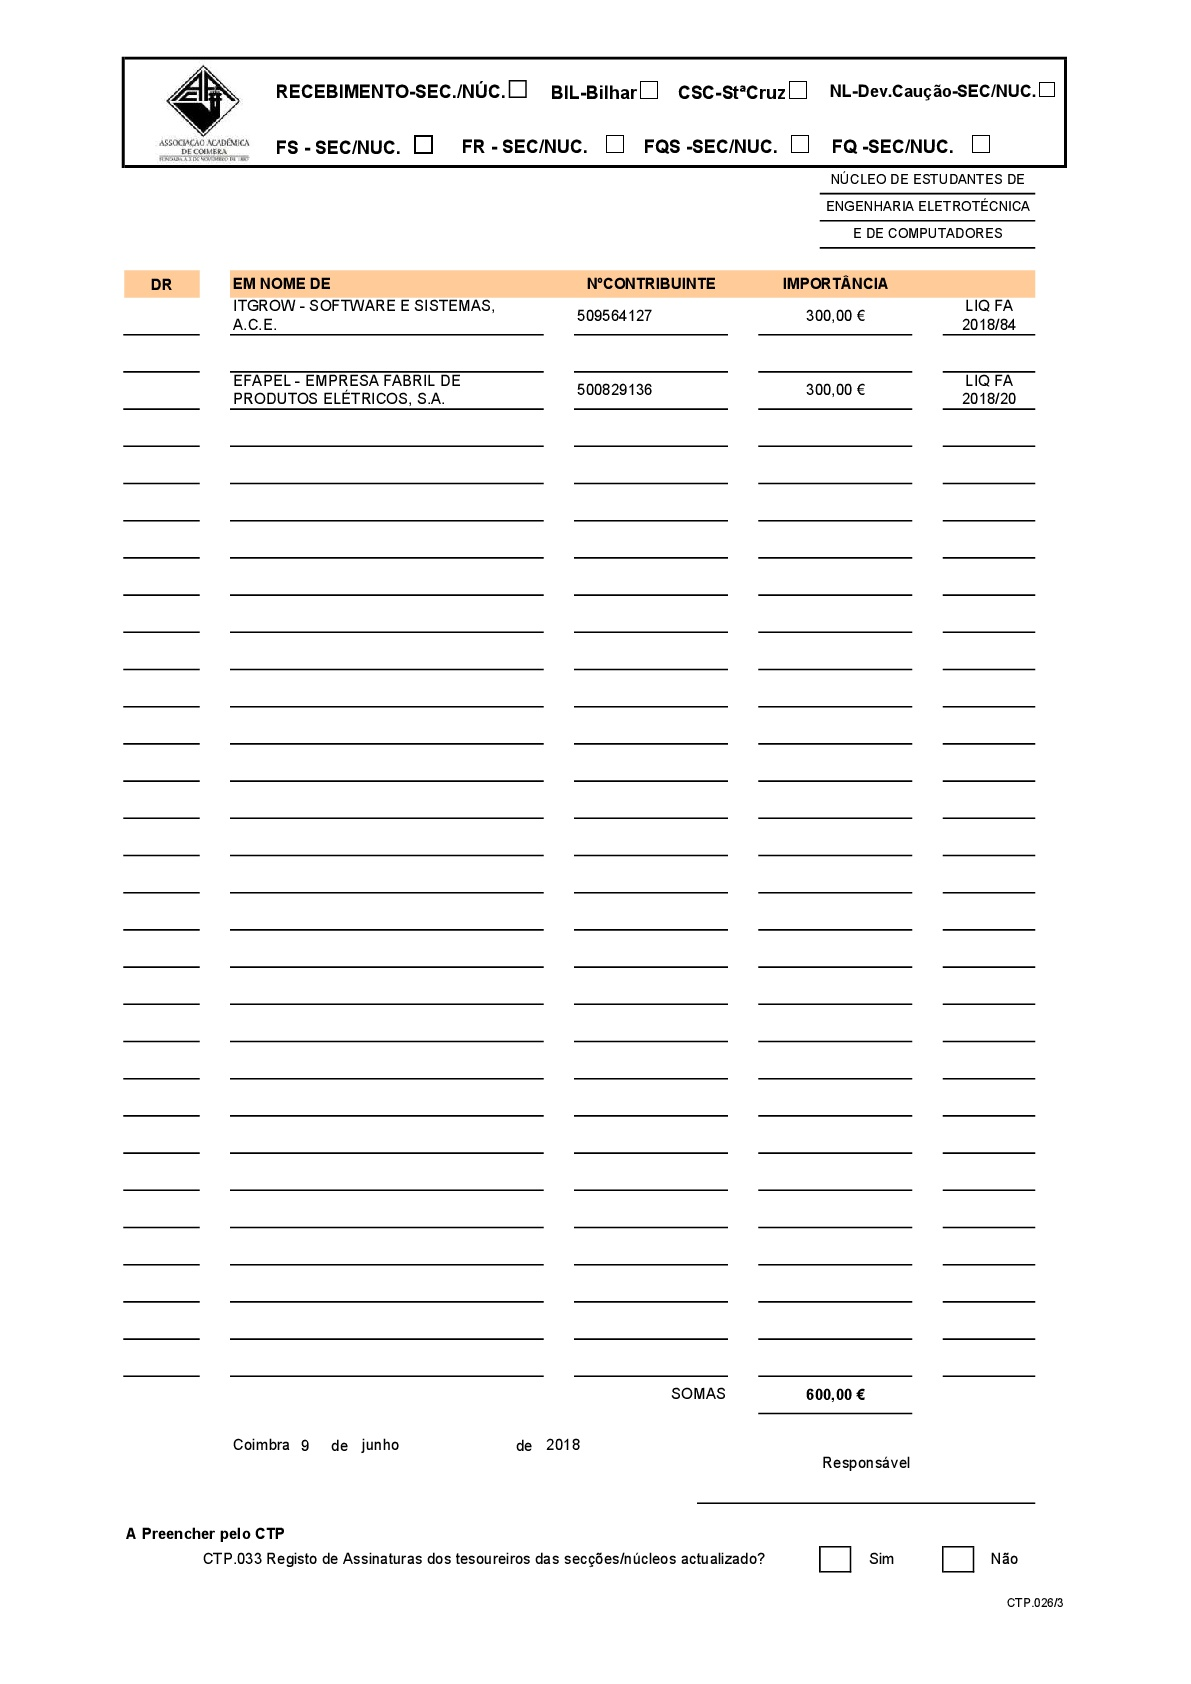
\includegraphics[width=\textwidth]{tesouraria/recibosFaturas}
        \caption{Pedido de recibos para faturas previamente emitidas.}
        \label{fig:Tesouraria-recibosFaturas}
    \end{subfigure}
    ~
    \begin{subfigure}[t]{0.3\textwidth}
        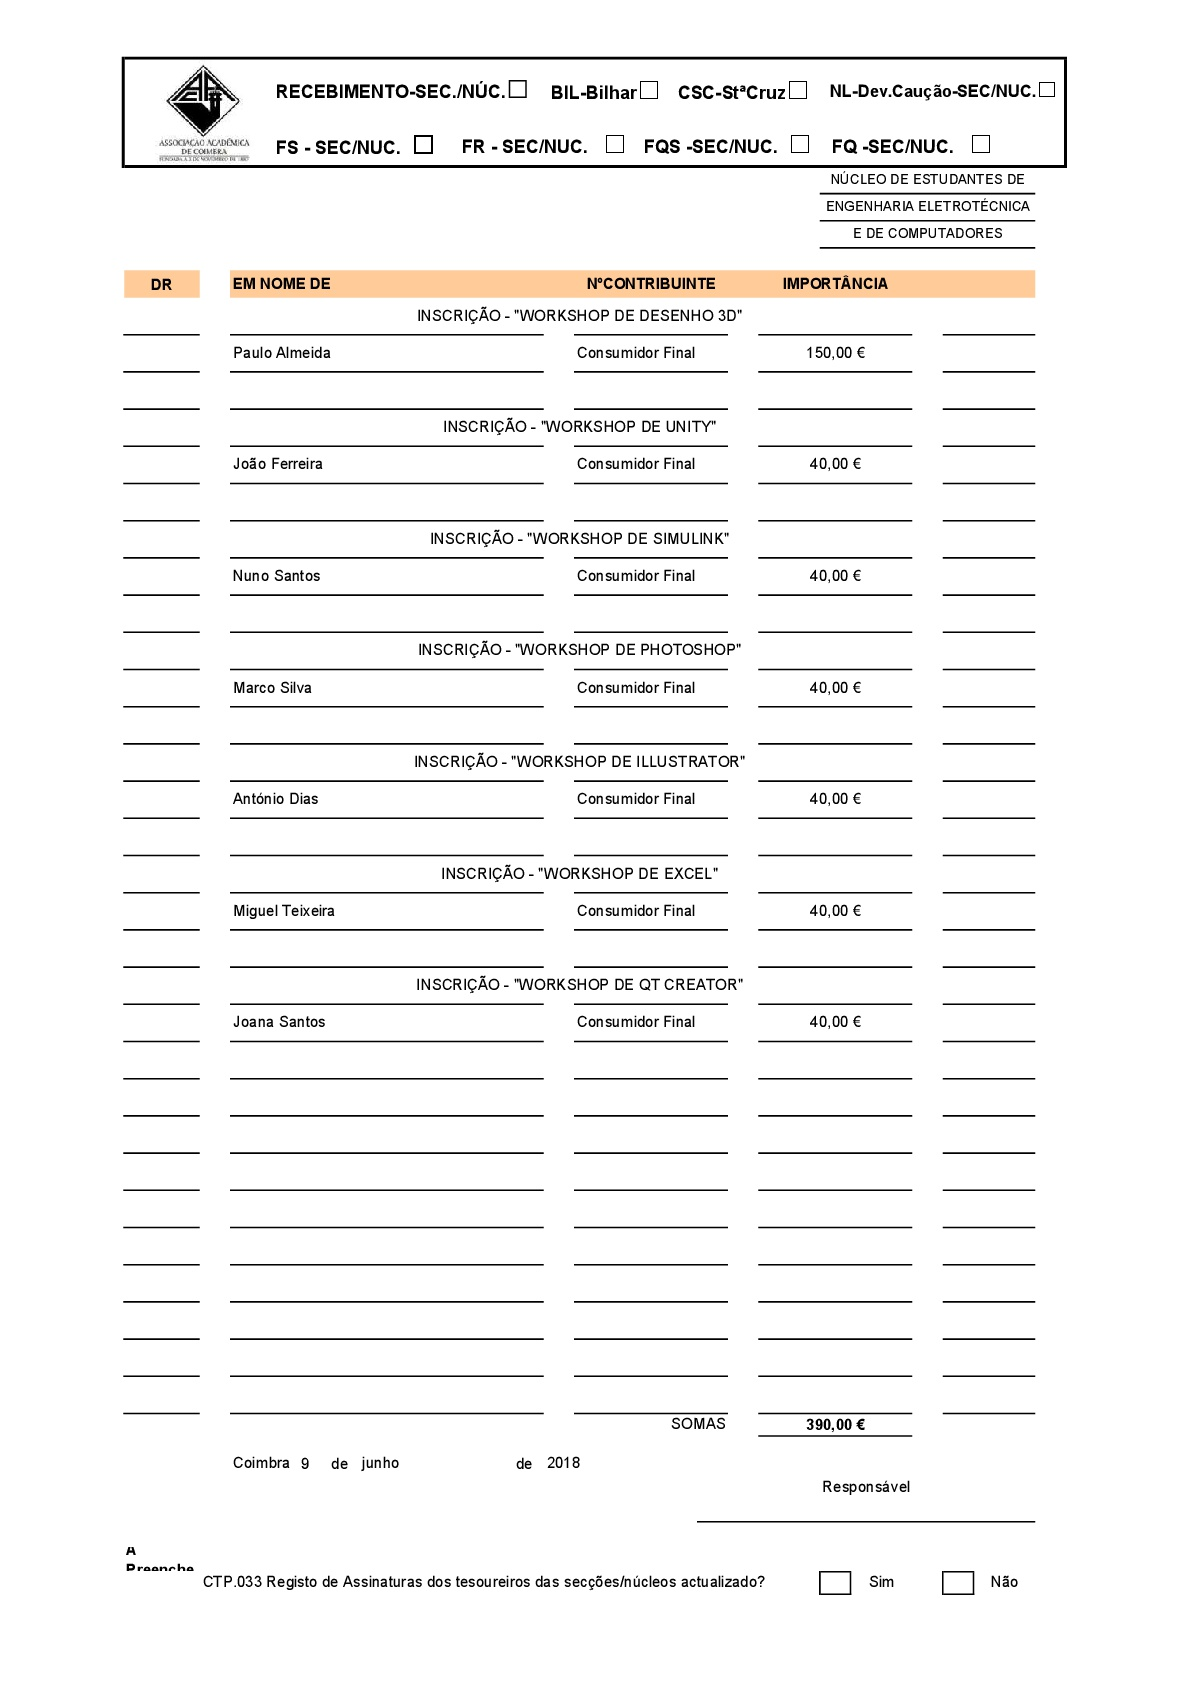
\includegraphics[width=\textwidth]{tesouraria/recibosInscricoes}
        \caption{Pedido de recibos para inscrições em atividades.}
        \label{fig:Tesouraria-recibosInscricoes}
    \end{subfigure}
    ~
    \begin{subfigure}[t]{0.3\textwidth}
        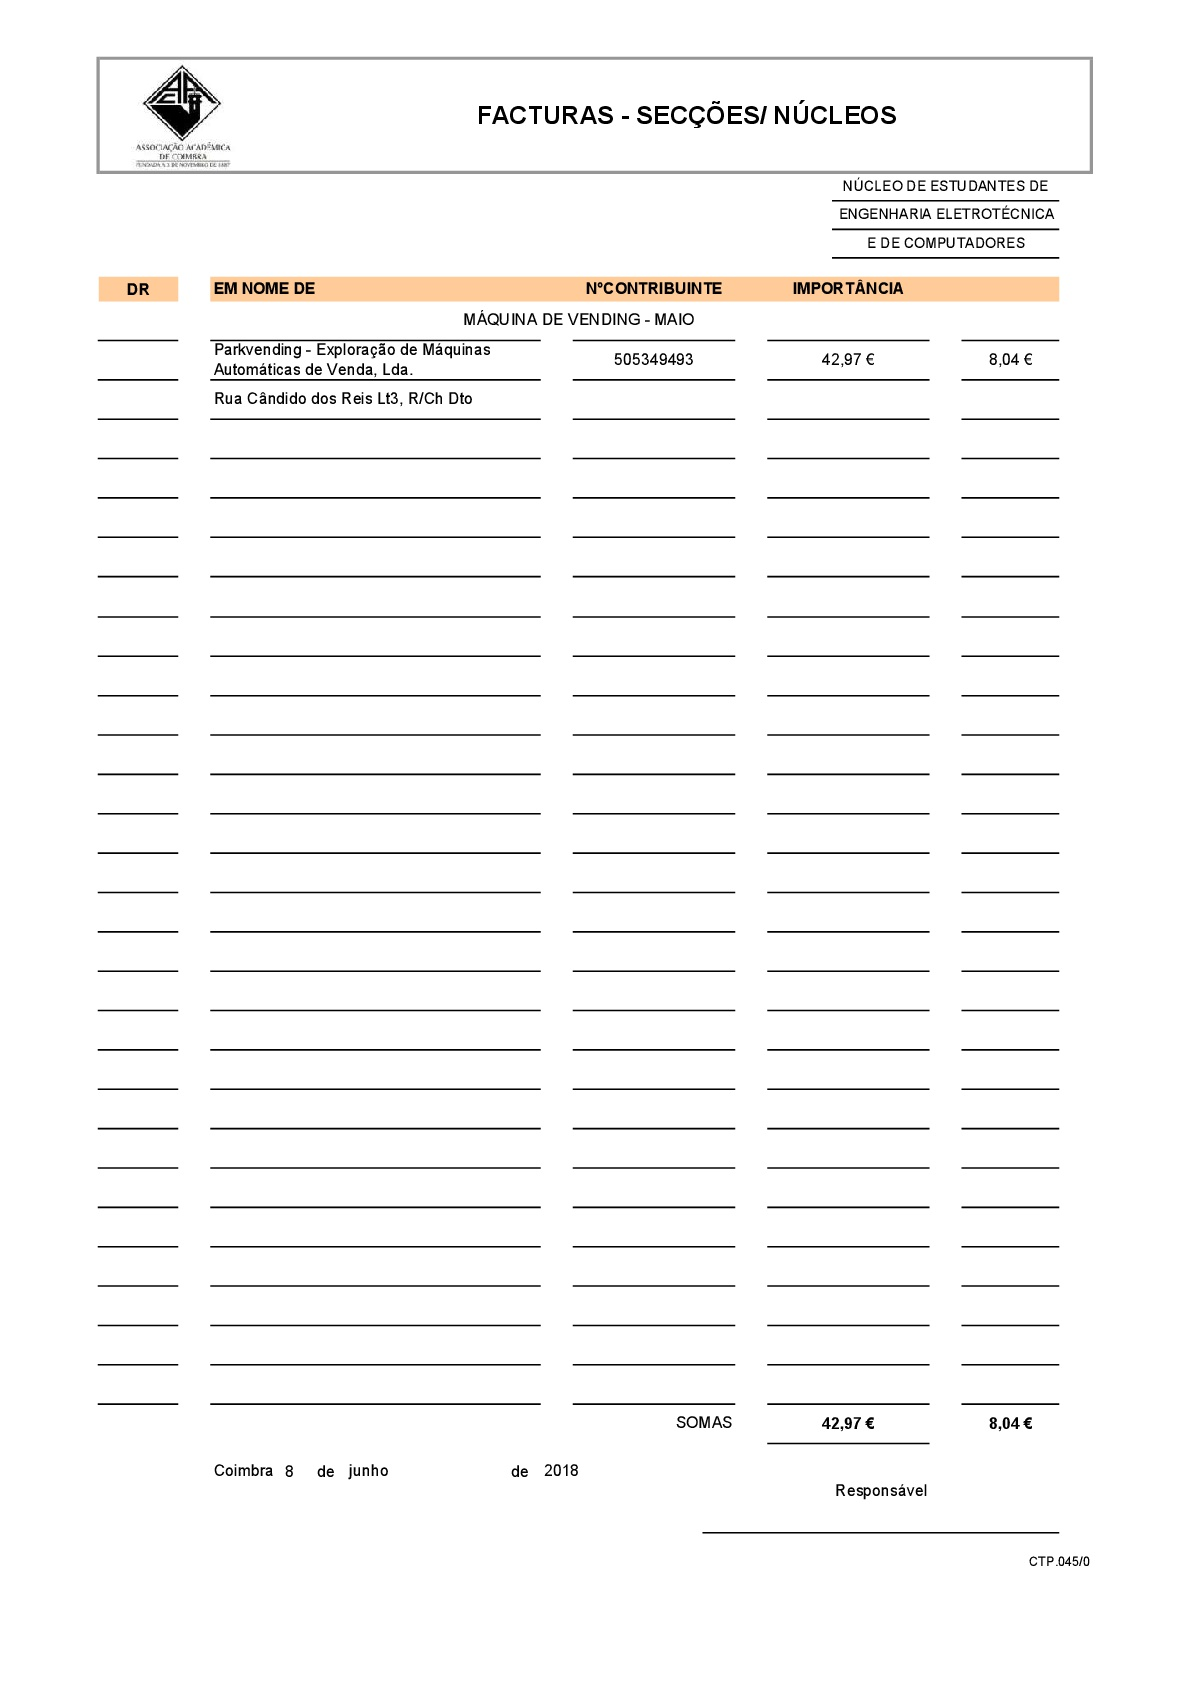
\includegraphics[width=\textwidth]{tesouraria/faturas}
        \caption{Pedido de faturas para pagamentos por realizar.}
        \label{fig:Tesouraria-faturas}
    \end{subfigure}
\end{figure}

\ifthenelse{\boolean{biblia}}
{ % TRUE
Exceto se pedido explicitamente pela pessoa, é recomendável agrupar os recibos das inscrições em atividades como "Consumidor Final"\space num recibo único para uma só pessoa, desde que o valor não ultrapasse os 199,99€, evitando a emissão de documentos inúteis. A partir do valor indicado, terão que ser emitidos múltiplos documentos até esse valor. No caso de pessoas que pedem o \acrshort{nif}, é obrigatório emitir individualmente cada recibo. Estes recibos pedidos explicitamente ou com o \acrshort{nif} devem ser entregues à pessoa, pelo que no decorrer do mandato, foram enviadas sempre digitalizações desses documentos por email, que poderão mais tarde levantar no Núcleo, caso o pretendam.
}
{ % FALSE
}

Quanto às faturas e recibos para empresas, cada empresa tem um método de trabalho distinto, pelo que para algumas empresas bastará enviar o documento digitalmente, enquanto que noutros casos é preciso enviar o mesmo por correio. Neste último caso, recomenda-se o aproveitamento dos modelos de carta e de envelopes já criados, adaptando apenas para o caso específico em questão. Recomenda-se ainda o envio da carta por correio registado, tendo assim sempre uma prova do envio da mesma, apesar dos custos associados a isso.

No caso de patrocínios em géneros, algumas empresas podem pedir um comprovativo desse apoio, como foi o caso do Pingo Doce este ano. Contudo, há que frisar que, no caso do Pingo Doce, das duas vezes que tal ocorreu, o mesmo homem pedia uma fatura dos apoios, o que implicaria pagar o \acrfull{iva}, contudo basta um documento certificativo emitido pelo \acrshort{ctp}, tal como será explicado caso seja feito esse pedido no gabinete do \acrshort{ctp}.

Por fim, há ainda o template de comprovativo de pagamento, que nunca chegou a ser utilizado este mandato. A utilização deste modelo chegou a ser pensado na altura do \acrshort{ene3}, pois houve devolução de inscrição a duas pessoas, contudo não se chegou a preenchê-lo dado que ainda não tinham sido emitidos os recibos dessas inscrições, pelo que a devolução anulou de imediato o valor recebido dessa pessoa.

Para que o preenchimento das informações dos documentos de Tesouraria, nomeadamente faturas, ficassem corretamente preenchidos e com os valores corretos, foi criado um modelo de faturação para simplificar o processo e permitir que, caso haja algum erro, a culpa seja tendencialmente da empresa. Este documento pede todo o tipo de informações necessárias, mas recomenda-se algumas alterações, nomeadamente na secção do montante do apoio para explicitar se o \acrshort{iva} está incluído, ou não, nesse valor.

\ifthenelse{\boolean{biblia}}
{ % TRUE
% ==========================
% # Gestão de caixa        #
% ==========================

\subsubsection{Gestão de Caixa}

Para além do cofre no \acrshort{neeec}, existe a caixa disponível para as vendas internas do Núcleo. Infelizmente, como esta é de acesso livre, ela tende a ser das maiores fontes do problema na gestão financeira do Núcleo. Esta caixa, até ao mandato anterior (2016/2017) tendia a ser um conjunto de várias caixas simples onde estavam guardadas algumas moedas para facilitar os trocos das pessoas, não havendo qualquer tipo de registo sobre o que era vendido, dependendo sempre da boa-fé das pessoas. Enquanto o único produto a ser vendido no \acrshort{neeec} era o café, era sempre possível verificar se os valores não estavam a ser aldrabados por uma contagem das cápsulas de café que ainda existiam em comparação com a contagem anterior. Contudo, mesmo nesta situação, bastava existirem cápsulas que estavam estragadas ou eventos que necessitavam de café para a contagem "descarrilar"\space e ser quase impossível manter um registo sobre o valor que devia existir. Além disso, ao misturar estes valores com os valores em dívida que eram permitidos para os membros do Núcleo, esta tarefa tendia a complicar bastante.

Inicialmente, neste mandato, mantivemos essa estratégia, tendo apenas unido tudo numa única caixa, dado que não era uma prioridade alterar isso, desde que as contagens não tivessem problemas. Contudo, como passámos a ter o frigorífico do Núcleo, começámos a vender também águas frescas e aproveitámos para vender algumas minis que tinham sobrado de eventos, pelo que as contagens simples se tornavam bastante tediosas e obrigava a um esforço redobrado para manter um registo quando alguns dos materiais desaparecia por causa de eventos. Para evitar essa situação, procurámos arranjar uma solução que permitisse as pessoas registarem o que tinham consumido e o método de pagamento, para além de permitir identificar movimentos de produtos utilizados em eventos. A solução inicial passou por uma folha de registos localizada por cima da caixa para que todas as pessoas vissem a sua existência e não se esquecessem de a preencher, contudo, mesmo assim, ainda demorou até que todas as pessoas se habituassem a este sistema, pelo que, apesar de reduzir significativamente os problemas que havia, acabou por criar outros, além do esforço que era analisar cada linha da folha de registos, ainda para mais preenchida à mão. Contudo, acreditávamos na altura que apostar num registo informático iria provocar ainda mais esquecimentos que o registo em folha, o que não iria resolver nenhum dos problemas que existiam. Mais tarde, o sistema mudou para um registo informático online (interno.neeec.pt), que, dado que as pessoas já estavam habituadas ao registo na folha, não provocou mais esquecimentos que os que já haviam com a folha. Supostamente esta plataforma facilitará bastante a gestão quando todas as funcionalidades pedidas para a parte de contabilidade estiverem concluídas, o que ainda não aconteceu, pelo que ainda mantém o mesmo nível de trabalho que a folha de registos tinha.

% ==========================
% # Como fazer caixas      #
% ==========================

\subsubsection{Como Fazer Caixas para Atividades}

Fazer caixa de trocos para as atividades do Núcleo é algo relativamente simples de fazer, mas que nem toda a gente é capaz, infelizmente. Esta deve ser pensada atempadamente para evitar confusões que ocorrem quando esta é feita à pressa e deve ser feita em função do preçário que esse evento terá. Por exemplo, se os preços a cobrar na atividade nunca envolvem moedas de 1, 2 e 5 cêntimos, estas serão desnecessárias para a caixa, exceto se existirem poucas moedas de 10 cêntimos, que são facilmente compensadas por estas, contudo será de evitar, pois cria um peso desnecessário na caixa.

Outra forma de analisar o precário, é pensar nas situações mais comuns de trocos que serão necessários. Por exemplo, numa febrada, as febras poderão ser vendidas a 1,20€, pelo que é frequente as pessoas pagarem os seguintes montantes: 1,20€; 1,50€; 2€; 2,20€; 5€, 10€. Desta forma, serão necessárias várias moedas de 10 e 20 cêntimos para quase todos os casos, de 50 cêntimos para o segundo e terceiro casos, de 1 euro para o quarto caso e assim sucessivamente. Ainda neste exemplo, como às vezes acontece não existirem moedas de 10 cêntimos suficientes, pode ser necessário ajustar o preço para 1,30€, evitando problemas com trocos.

Regra de ouro a fazer caixas: os montantes pequenos somados dão montantes grandes, contudo os montantes grandes não podem ser partidos para os montantes mais pequenos.
}
{ % FALSE
}

% ==========================
% # Montepio Geral         #
% ==========================

\subsubsection{Montepio Geral}

A \acrshort{aac} tem há alguns anos um acordo com a Caixa Económica Montepio Geral, pelo que todas as contas da \acrshort{aac} (secções, núcleos de estudantes, Queima das Fitas, etc.) têm uma conta neste banco, sendo as estruturas impedidas de abrir conta noutro banco, sendo mesmo impedidas de receber qualquer tipo de apoio doutras instituições bancárias, mesmo que estes apoios sejam solidários, por exemplo. A conta do \acrshort{neeec} tem quatro titulares da conta: o Presidente e Tesoureiro do Núcleo e o Presidente e Administrador da \acrshort{dg}. Sendo assim, sempre que um destes titulares precisa de ser alterado (novos órgãos dirigentes de cada uma das estruturas, por exemplo), é cobrada uma taxa pelo banco.

A gestão da conta é bastante simples, estando disponível a interface web e a interface por telemóvel, sendo interfaces completamente naturais para este tipo de instituições. Cada titular tem o seu acesso personalizado e tem um cartão matriz que serve para confirmar as transações (estas são enviadas por correio e terão de ser levantadas no edifício da \acrshort{aac}). Todos os movimentos financeiros na conta do Montepio Geral têm que ser autorizados por dois dos titulares da conta (suspeitamos que esta regra se deva a abusos que tenham existido quando apenas um dos titulares pudesse fazer o que bem entendia), o que impede a existência de um cartão bancário de acesso direto à conta. No final do mandato, para evitar pagamentos através de contas de terceiros que seriam posteriormente transferidos para a conta dessa terceira entidade, pedimos o cartão pré-pago da conta (este teve um custo de 6€), que permite ser carregado com um valor até 2000€. Esse carregamento terá que ser aceite sempre por dois titulares da conta, pelo que evita (parcialmente) o problema da existência de cartão de acesso direto à conta.

Todos os meses o banco emite um extrato combinado da conta, que pode ser transferido através do site. Este extrato é o usado pela Susana do \acrshort{ctp} para verificar os valores da conta, pelo que cada movimento terá que ser justificado.

% ==========================
% # Orçamentos e Execuções #
% ==========================

\subsubsection{Orçamentos e Execuções}

A criação de orçamentos é uma das principais tarefas do Tesoureiro, permitindo estabelecer uma barreira quanto aos gastos que o evento possa ter, as receitas que é necessário atingir para esses mesmos gastos e o lucro da atividade. O lucro da atividade não precisa de ser sempre positivo, desde que haja a definição inicial de que tipo de atividades poderão, ou não, ter lucro/prejuízo em nome da sustentabilidade tanto da atividade como do Núcleo.

A criação de um orçamento, para qualquer tipo de atividade, é, provavelmente, das tarefas mais complexas, principalmente quando o histórico de gastos e receitas das atividades é inexistente ou manifestamente escasso. Nestes casos, é necessário ter alguma noção do que a atividade requer, ou não, e os custos ou receitas possíveis que é possível ter com esses requerimentos, o que é especialmente difícil quando não se sabe um valor aceitável para esses requerimentos. Para tal, é necessário conversar muito bem com o organizador da atividade para perceber o que vai ser realmente feito e este deve saber transmitir valores aceitáveis para esses requerimentos, contudo é necessário ter sempre alguma desconfiança (saudável) e realizar uma pesquisa própria sobre esses valores.

Durante este mandato, foram iniciados os passos para uma construção frequente de orçamentos, tendo sido realizados orçamentos principalmente para as atividades grandes do Núcleo, nomeadamente \acrshort{ene3}, Bot Olympics e Gala Ohms D'Ouro. Quando foi possível, foi feita uma pesquisa sobre os orçamentos que já existiam e as discrepâncias para os valores reais que apresentaram para que fosse possível discernir os valores a definir, pelo que se aconselha uma pesquisa por esses documentos feitos. Nos ficheiros das execuções financeiras dessas atividades, foi também ambição disponibilizar o valor da discrepância que se verificou para facilitar o trabalho futuro.

% ==========================
% # Regimento Interno      #
% ==========================

\subsubsection{Regimento Interno}

As regras de tesouraria e contabilidade que o \acrshort{ctp} impõe, apesar de não serem muito complexas, são muito fáceis de serem esquecidas, principalmente pelas pessoas que não estão a par deste tipo de assuntos. Por isso, recomenda-se a criação de um regimento interno, bastante simples, onde são explicitadas todas as regras que as pessoas têm que cumprir, nomeadamente, quanto às compras que as pessoas fazem e que precisam que o \acrshort{neeec} pague. As principais regras a referir deverão ser:
\begin{itemize}
    \item O pedido de despesa obrigatório ao Tesoureiro (com as devidas exceções que terão que ser aceites por este);
    \item A presença do \acrshort{nif} tanto da \acrshort{aac} (500 032 173) como do vendedor;
    \item O nome a colocar nas faturas (Associação Académica de Coimbra - NEEEC);
    \item As regras quanto aos gastos com combustível;
    \item A necessidade das faturas de reservas (reservas de espaços como o local da Gala Ohms D'Ouro) conterem o número de pessoas referentes à reserva.
\end{itemize}

% ===============================
% # Relacionamento com empresas #
% ===============================

\subsubsection{Relacionamento com Empresas}

As empresas com que lidamos normalmente têm métodos muito distintos de se relacionar connosco, pelo menos, a nível de Tesouraria. Enquanto que algumas empresas requerem que se envie a fatura do apoio por correio antes destas pagarem, outras basta apenas enviar uma digitalização dessa fatura por email. Chegou mesmo a acontecer, apesar de ter sido um caso único, ter havido uma empresa a pagar antes de ter sido sequer pedida a fatura. Neste caso, é necessário ter uma comunicação estreita com a pessoa que está a tratar dos patrocínios de cada evento, para que estas informações de como lidar com a empresa em questão não se perca, dado que acontece frequentemente as empresas mudarem o seu método de trabalho (aconteceu este mandato com a Critical Software/itGrow, que passou a requerer o envio por correio das faturas) e é preciso saber o que cada uma precisa.

Durante este mandato, houve duas formas de lidar com o envio de faturas para empresas: na maior parte das vezes, o processo de arranjar o patrocínio pertencia a uma pessoa e depois o processo de faturação caía todo sobre o Tesoureiro, enquanto que noutros casos, o Tesoureiro era apenas responsável por pedir a fatura que depois enviava à pessoa responsável pelo pedido de patrocínio que tratava de enviar para a empresa. 

Nota pessoal do Tesoureiro: preferi a primeira situação, porque permitiu manter um histórico de como lidar com cada empresa (existe mesmo um histórico dos modelos de pedidos de informação preenchidos pelas empresas na pasta da Tesouraria) e assim saber lidar diretamente com a empresa caso surgisse algum problema, que normalmente apenas surge numa fase final da preparação do evento ou até mesmo depois do evento e que a pessoa que fazia a ligação anteriormente poderá já não estar disponível para solucionar.

Um problema recorrente ao lidar com empresas é a confusão gerada pelo facto de todas as estruturas da \acrshort{aac} partilharem um \acrshort{nif} comum, principalmente nas empresas mais organizadas que têm um software de gestão de contabilidade e criam fichas de clientes que apenas permite criar um ficha por \acrshort{nif} associado. Desta forma, pode acontecer as empresas contactarem as pessoas erradas para resolver algum problema ou, mais frequentemente, transferirem os apoios monetários a atividades para outras estruturas da casa. Neste campo, são excelentes exemplos a EFAPEL que apoia a Secção de Basquetebol, transferindo sempre o dinheiro para estes, e a ITGrow que transferia sempre para o \acrshort{nei} o dinheiro e atualmente transfere sempre para nós, mesmo quando o dinheiro não é para nós. Nestas situações é necessário descobrir para onde o dinheiro foi transferido (por exemplo, colocar no multibanco o NIB de forma a saber o titular da conta para onde foi transferido o dinheiro) e contactar as estruturas em causa, solicitando a transferência do dinheiro para a conta bancária correta.

\ifthenelse{\boolean{biblia}}
{ % TRUE
% ===============================
% # Relacionamento com o Polo 2 #
% ===============================

\subsubsection{Relacionamento com o Polo 2}

O Polo 2, cujas atividades são discutidas em pormenor na secção \ref{sec:polo2}, é uma pseudo-associação dos Núcleos do Polo 2, cuja atividade se tem cingido muito à componente lúdica. A atividade principal do Polo 2 tem sido o Mega-Convívio do Polo 2, integrada na Semana de Receção ao Caloiro e que neste mandato teve mais de 10000€ de receitas e de despesas e, pela primeira vez em algum tempo, apresentou lucro, bastante residual (cerca de 11€ por núcleo). Dado o elevado montante de despesas a assumir numa fase muito inicial da atividade, é costume cada Núcleo entrar com um valor para a caixa do evento que depois lhe é devolvido (integralmente apenas caso a atividade dê lucro) e cujo montante varia com a disponibilidade que cada Núcleo dispõe, com montantes na ordem dos 500€. Este valor, nos últimos anos, dada a situação da dívida, era incomportável pelo nosso Núcleo, pelo que entrámos apenas com 250€ nestes últimos dois anos.

O Polo 2 tem por hábito não declarar oficialmente quase nenhuma das despesas e receitas que o evento tem, pelo que o valor de caixa de entrada tem que ter origem nos valores do saco azul. Tal como explicado anteriormente, consideramos que a existência de um saco azul é contraproducente para a saúde financeira do Núcleo (permite movimentos desconhecidos das autoridades competentes) e impede uma transparência do Núcleo que afasta muitos dos seus sócios. Desta forma, fizemos questão de eliminar o saco azul que existia no nosso Núcleo, impedindo que possamos comparticipar esta atividade de forma escondida da \acrshort{aac}, pelo que é imperativo agilizar o processo de transparência desta associação.
}
{ % FALSE
}
}
{ % FALSE
}

% =============================
% # Organização de Atividades #
% =============================

\subsection{Organização de Atividades}

A interação e interligação das funções dos diversos membros quer da Direção, quer dos CGs está inerente à organização de cada atividade do Núcleo. A projeção e idealização está a cargo de cada Pelouro com o auxílio do responsável da Direção por esse Pelouro. Após definição dos objetivos para cada atividade, o CG deve estipular com o Secretário a calendarização e registos de informações relevantes bem como a abertura de inscrições, reunir com o Tesoureiro para planeamento do orçamento e custo por participante e reunir com o Administrador para eventuais compras e organização logística necessária para fazer uso do material do Núcleo. O estabelecimento de todos os contactos deve ser realizado via Slack, de modo a assegurar o registo apropriado e consequentemente proporcionar uma melhor organização da atividade. Deve ser também feito um pedido de imagem, no formulário respetivo, para que o Pelouro da Imagem e para que os responsáveis pela Comunicação possam articular o seu trabalho e divulgar o evento com a devida antecedência. Por todas estas questões, é indispensável uma boa articulação e gestão de toda a equipa. Os Colaboradores têm como papel a organização e execução de todas as tarefas no decorrer da atividade, sendo que todos os membros do Núcleo se devem disponibilizar para auxílios pontuais. Toda a articulação na organização das iniciativas é orientada pelo Presidente do \acrshort{neeec}. É também importante a criação e divulgação prévia e atempada das escalas necessárias para a execução da atividade quando o staff do Pelouro em questão não tem capacidade para, sozinhos, assegurarem o evento.

Após a concretização da atividade, o CG do Pelouro é também responsável pela emissão de certificados e justificação de faltas, caso se aplique, e a arquivar as fotografias registadas no evento para uso posterior. Os responsáveis da Comunicação devem também fazer a divulgação do evento através de uma foto ou outra ou de um álbum, caso se trate de um evento de âmbito mais social.

% ===========================
% # Comissões Externas      #
% ===========================

\subsection{Comissões Organizadoras}

Para além das atividades desenvolvidas pelos pelouros ou pela Direção existem atividades de maior dimensão que necessitam de uma comissão organizadora. No presente mandato foram criadas comissões para a realização do \acrshort{ene3}, da \acrshort{ugf}, do Bot Olympics, da Gala Ohms D’Ouro e das celebrações dos 20 anos do \acrshort{neeec}. O mês solidário e respetiva componente solidária foram também organizadas por uma pequena comissão externa, de reduzida dimensão orientada pelo João Bento e pela Ana Calhau.

No mandato anterior (2016/2017), aquando do teambuilding, cada membro do Núcleo pôde dizer em que evento gostaria de participar (Bot Olympics ou Gala Ohms D'Ouro). Essa situação foi referida para quem estava na sala de estar da casa onde decorreu o teambuilding e voltou a ser mencionada dias mais tarde na sala do Núcleo. Desta forma as pessoas só puderam ocupar uma das comissões e houve comissões que tiveram várias pessoas desnecessárias e falta de pessoas com determinadas competências. Facilmente, quer numa comissão, quer noutra, as pessoas abandonaram as mesmas. No caso da gala, aquando da reta final da organização da mesma, já só a Presidente da altura estava a organizar a gala em conjunto com outra pessoa.

Este ano, optámos por criar as comissões em reunião de Direção, convidando as pessoas a fazer parte das mesmas. Achamos que esta organização deu resultados muito positivos, uma vez que permitiu uma melhor gestão de toda a equipa, divisão dos membros pelas várias comissões e atribuição de membros às competências que melhor desempenham. Podemos, no entanto, ter deixado de fora alguns membros que potencialmente poderiam ter ajudado bastante mas dos quais não tínhamos feedback suficiente para considerarmos a sua inserção nas comissões evitando, contudo, que vários membros que pretendiam juntar-se mas que não iriam fazer nada ocupassem lugares. Na totalidade dos casos, consideramos que esta medida melhorou em muito a qualidade do trabalho desenvolvido comparado com os métodos de seleção aplicados em mandatos anteriores.

\subsubsection{UGF}

Esta comissão foi presidida, ao início, pelo CG da Cultura e Lazer, Carlos Abegão, que ficou como Coordenador do evento. Após entrarmos em contacto com os outros Núcleos envolvidos (\acrshort{nei} e \acrshort{neemaac}), ainda em julho, convidámos várias pessoas a fazer parte desta comissão. O Coordenador não gostou que tivéssemos convidado pessoas sem ser ele a decidir, o que apesar de compreensível, teve como intuito uma gestão equilibrada de toda a equipa do \acrshort{neeec} para se saber como dividir a equipa para os vários eventos que iríamos ter. Contudo, ao convidarmos membros numa altura em que ainda quase ninguém tinha tido a oportunidade de mostrar trabalho para o Núcleo fez com que convidássemos algumas pessoas que não tinham as qualidades necessárias para o evento. Além disso, a saída do CG da Cultura e Lazer fez com que o Administrador do Núcleo passasse a ser Coordenador deste evento, criando entropia na equipa dado o período de ambientação que este teve de ter para se inteirar do evento. Também a própria estrutura da Comissão Organizadora, já com os vários Núcleos, em que estes (\acrshort{neemaac}) só pretendiam ter alguns pelouros em alturas mais tardias, fez com que, ao longo do ano, fosse entrando e saindo gente da organização o que é péssimo para as pessoas se ambientarem ao evento e estarem a par das várias decisões já tomadas desde o início da organização.

\subsubsection{Bot Olympics}

Em outubro, foram criadas, em simultâneo, em reunião de Direção, as comissões organizadoras do Bot Olympics e da Gala Ohms D'Ouro. Uma vez que o Bot Olympics foi realizado em conjunto com o \acrfull{cr} já sabíamos que áreas teríamos que preencher com pessoal do \acrshort{neeec}. Desta forma, ao serem selecionadas as pessoas, estas foram logo apontadas para a área onde iriam trabalhar. Em paralelo, foram escolhidos três Coordenadores que não ficaram responsáveis por nenhuma área do evento. Esta comissão resultou muito bem tendo sido apenas necessário substituir um dos responsáveis (o responsável pelo contacto às escolas) tendo este sido substituído pelo Presidente do Núcleo já bastante tarde (em dezembro) e tendo um dos responsáveis pelos patrocínios por parte do Clube de Robótica abandonado a comissão, algo que já tinha sido previsível e contemplado um plano alternativo pelo que não trouxe problemas.

\subsubsection{Gala Ohms D'Ouro / 20 Anos do NEEEC/AAC}

A criação da comissão para a gala contemplou de imediato a tarefa de criar a VI edição da Gala e planear todas as celebrações do 20º aniversário do \acrshort{neeec}, uma vez que as datas e a temática eram bastante próximas. Como é habitual na gala, o Presidente do Núcleo foi um dos Coordenadores do evento tendo, este ano, sido acompanhado pela Vânia Silva. Tendo em conta o maior trabalho que se previa foram convidadas várias pessoas, num número maior do que o habitual para este evento. Esta comissão resultou muito bem tendo apenas havido duas alterações: a Elisabete Santos, que entrou após ter saído da \acrshort{dg}, para apoiar na história do Núcleo e a entrada do Tiago Baltazar, um dos apresentadores do evento. De realçar, no entanto, que havendo uma estrutura completamente nova na gala e ainda mais diferente tendo em conta a celebração do aniversário, houve várias pessoas que tiveram de ser elucidadas sobre as suas tarefas e como funcionaria o trabalho para as mesmas, tendo a comissão um período grande de adaptação até ter entrado no seu pleno de trabalho, em algumas áreas. Dado que esta edição da gala celebrou o aniversário do Núcleo, teve uma equipa maior que o habitual que não será necessária em futuras edições da mesma.

\subsubsection{ENE3}

Este evento começou a ser organizado ainda no início do mandato anterior, tendo, por isso, uma comissão já organizada no início do mandato 2017/2018. No entanto, foi necessário acrescentar vários elementos do novo mandato do Núcleo e o Presidente e Vice-Presidente do Núcleo tiveram de passar a ser Coordenadores do evento, algo que não foi feito com tanto planeamento como aconteceu nas atividades referidas anteriormente, mas que acabou por correr bastante bem por se tratar de um evento que decorreu muito antes das restantes atividades.

\subsubsection{Outros}

Existem ainda vários outros eventos de considerada dimensão, alguns do Polo 2, outros do Pelouro das Saídas Profissionais, por exemplo, que não tiveram comissões externas, mas que envolveram o trabalho de vários pelouros em conjunto, de acordo com os métodos laborais estipulados para o Núcleo.


% ==========================
% # Regalias dos Membros   #
% ==========================

\subsection{Regalias dos Membros}

Cada um dos Pelouros do \acrshort{neeec} tem uma equipa atribuída que, em conjunto, permitem o desenvolvimento do trabalho do \acrshort{neeec} avançar. Além das funções de cada Pelouro, toda a equipa colabora nos eventos de âmbito geral do Núcleo ou em atividades de maior dimensão como foi o caso do Encontro Nacional de Estudantes de Engenharia Eletrotécnica ou do Bot Olympics.

Desta forma, e por sugestão de antigos dirigentes da casa, a Direção do \acrshort{neeec}, tentou estudar a possibilidade de atribuir algumas regalias, principalmente aos Colaboradores que não têm qualquer tipo de benesse no seu trabalho, fazendo com que sintam que o seu trabalho seja compensado. É ainda de realçar que muitos dos Colaboradores, dado o seu trabalho, acabam por assumir funções de elevada responsabilidade e carga horária pela qualidade do trabalho que prestam.

Foram solicitados suplementos ao diploma para a organização, staff e participantes de atividades de maior dimensão tais como o Bot Olympics, o Encontro Nacional de Estudantes de Engenharia Eletrotécnica e a Feira de Emprego e Empreendedorismo. Contudo, fica em falta o reconhecimento ao trabalho geral de todo o mandato e dos pelouros em si.

Assim, após análise em reunião, a proposta da Direção do \acrshort{neeec} foi criar uma classificação que tentou, de forma o mais justa possível, identificar quem é de facto ou não merecedor de algum tipo de benesse e em que medida. Para tal, selecionaram-se vários critérios, abaixo descritos, de forma a avaliar o trabalho de todos os membros:
\begin{itemize}
\item Presenças na escala do Núcleo (30\%)\\
Desde setembro de 2017, a sala do Núcleo dispõe de um horário de atendimento, durante o período de aulas, entre as 10h e as 17h com encerramento para almoço entre as 13h e as 14h, com exceção das quartas-feiras à tarde e das sextas-feiras de manhã em que o Núcleo se encontra encerrado. Desta forma, todos os Coordenadores e Colaboradores devem ocupar um turno ou dois, respetivamente, de uma hora em cada semana. As presenças do mesmo são registadas em folha de presenças afixada na sala do Núcleo pelo Secretário. Quem não cumpriu um turno na escala tem falta e todas as semanas a escala pode ser alterada sendo que o Secretário só ao domingo à noite imprime a folha de presenças já com os nomes da escala dessa semana. Todos os Colaboradores que faltem à escala justificadamente têm a sua presença justificada desde que indiquem o motivo ao Secretário e este seja considerado válido. Os turnos que se sobrepõe a exames ou dias festivos (por exemplo, após a serenata da Queima das Fitas) não contam para as presenças.
A nota atribuída a este parâmetro é diretamente proporcional ao número de presenças na escala (Em 28 turnos, uma pessoa que tenha vindo a 14, terá 15\% nesta avaliação enquanto que quem veio aos 28 turnos terá 30\%).
\item Presenças em escalas de eventos (10\%)\\
Ao longo do mandato existem vários eventos gerais do Núcleo e eventos cuja capacidade logística transcende a capacidade do Pelouro que a organiza. Desta forma, é necessária a criação de escalas para esses eventos de forma a os organizar. Para este ponto foram analisadas as seguintes escalas: banca na semana das matrículas, dia da receção ao caloiro, \acrshort{f3e}, \acrshort{neeec} Open Day, Lanche Solidário, Mega Febrada do Polo 2, Mega Febrada Polo 2, Venda do Jantar de Curso, Noite de Fados, Visita à Ubiwhere, Bot Olympics, Nomeações dos Ohms D’Ouro, Votações dos Ohms D’Ouro, Ultra Gaming Fest, BeerOlympics Eliminatória, BeerOlympics Final e Peddy Tascas. Não foram considerados eventos onde as escolas foram restritas a apenas algumas pessoas (por exemplo, a Barraca da Festa das Latas que foi restrita a Coordenadores e quatro Colaboradores que foram convidados para tal). Foi também decidido dar-se uma percentagem de apenas 10\% a este aspeto uma vez que muitos eventos calham nos mesmos dias da semana e, dessa forma, as pessoas que não podem comparecer num também não poderão comparecer noutro que se realize no mesmo dia da semana.\\
A nota atribuída a este parâmetro é de 10\% para todas as pessoas que tenham feito 12 ou mais turnos por semestre, sendo a partir daí para baixo proporcional ao número de presenças.
\item Avaliação Individual (40\%)\\
Esta avaliação dada por cada Coordenador de Pelouro aos seus Colaboradores e dada pela Direção aos Coordenadores, pretende avaliar o trabalho dos mesmos para o bom funcionamento do Pelouro e para a qualidade do trabalho nele desenvolvido. Os CGs são avaliados pela Direção tendo em conta o seu desempenho na coordenação dos respetivos pelouros e nos resultados alcançados, no seu trabalho para o intuito do Pelouro e no respeito pelas formas de trabalho estabelecidas para a equipa no seu global.\\
A avaliação é feita numa métrica de 0\%, 20\% ou 40\%, respeitando assim três níveis. Caso um Pelouro tenha funcionado notoriamente mal, a Direção poderá intervir, alterando a classificação dada aos colaborados do Pelouro em questão.
\item Proatividade na comunicação (10\%)\\
Sendo a comunicação um dos pilares mais essenciais do Núcleo, entendemos que este deve ser também avaliado. Assim, os responsáveis da comunicação devem avaliar quem está sempre a colaborar na divulgação das atividades do Núcleo, quem o faz de vem em quando ou quem nunca o faz (quer através de passar a mensagem boca-a-boca, quer através da divulgação nas redes sociais, etc). Serão valorizadas as pessoas que são mais independentes nesta área em vez das pessoas que têm de ser constantemente chateadas para colaborarem neste campo.\\
A avaliação é feita numa métrica de 0\%, 5\% ou 10\%, respeitando assim três níveis.
\item Avaliação bónus (10\%)\\
Havendo vários aspetos não avaliados nos pontos anteriores, nomeadamente a proatividade das pessoas, a presença das mesmas para ajudar em atividades gerais como a remodelação dos espaços de estudo, a montagem das decorações de Natal, entre outros, a presença em reuniões, a proatividade na sugestão de ideias, a colaboração para o conteúdo do site do Núcleo, entre muitas outras, a Direção valoriza todos os membros que têm espírito de iniciativa e disponibilidade tentando assim avaliar os pontos que não foram avaliados nos pontos anteriores.\\
A avaliação é feita numa métrica de 0\%, 5\% ou 10\%, respeitando assim três níveis.
\end{itemize}
Tendo em conta os critérios de avaliação aqui descritos, as benesses pensadas pela Direção do \acrshort{neeec} foram as seguintes:
\begin{itemize}
	\item As avaliações inferiores a 50\% não têm qualquer tipo de benesse.
	\item As avaliações entre 51\% e 79\% têm os seguintes direitos:
      \begin{itemize}
      \item Menção na \acrshort{rga}
      \item Certificado de participação ativa assinado pelo \acrshort{neeec} e pelo \acrshort{deec}
      \end{itemize}
 	\item Avaliações superiores a 80\%:
      \begin{itemize}
      \item Menção na \acrshort{rga}
      \item Certificado de participação ativa assinado pelo \acrshort{neeec} e pelo \acrshort{deec}
      \item Inscrições nas atividades gratuitas (workshops)
      \item Cartas de recomendação (individuais e especializadas)
      \item Potenciais suplementos ao diploma
      \end{itemize}
\end{itemize}

Com estas avaliações, pretendeu-se atingir o patamar justo para todos os membros não prejudicando quem não colaborou da forma que devia para o mandato, uma vez que não deixamos de ser uma organização sem fins lucrativos, não profissional e feita de estudantes cuja principal atividade não é esta, mas valorizando todos aqueles que despenderam muito do seu tempo para trabalhar em prol desta casa.

É de notar que esta classificação foi positiva contudo as percentagens podem não ser as mais justas. No final do ano, o que verificámos é que a larga maioria dos casos foi extremamente justa tendo, no entanto, existido casos pontuais em que o resultado pode não ter sido o mais adequado, nomeadamente com a justificação de falta de preenchimentos de escala a quem tinha sobreposição de horários, fazendo com a classificação desses membros subisse de forma galopante comparando com os restantes. De notar que, de forma a não haver qualquer injustiça sobre os diversos casos, não houve uma única nota alterada, mesmo os casos que estavam perto da transição para o nível seguinte. De notar que as notas não foram divulgadas publicamente (por exemplo no canal geral do Slack) para evitar que se tratasse o Núcleo como se fosse uma cadeira mas, quem quis, pode saber as suas avaliações individuais.

\subsection{Representação do NEEEC/AAC}

Ao longo do mandato é frequentemente necessário representar o \acrshort{neeec} em ações de carácter diverso. Uma vez que pertencemos à \acrfull{aac}, a capa e batina deve ser utilizada sempre que se adeque, não só pelo Presidente e Vice-Presidente do Núcleo, mas por todos os que o representam (como aconteceu, por exemplo, nos 20 anos do Núcleo e na manifestação "Basta"). Apesar de no nosso Núcleo não ser habitual, existem vários Núcleos que mesmo em Reuniões Gerais de Alunos, a Mesa do Plenário bem como a Direção se apresentam de capa e batina. Em outras atividades como cerimónias de abertura de eventos é também essencial a apresentação de capa e batina. Este é um hábito que, principalmente os membros fora da Presidência, preferem abdicar o que, no nosso ver, é completamente errado e desprestigia o símbolo da Academia que representamos. Noutros casos como a visita a empresas, reuniões, etc., deve ser adotado um visual correto podendo-se fazer uso do merchandising do \acrshort{neeec} para tal, de forma a promover a imagem do mesmo.

É também importante manter o \acrshort{neeec} representando em todas as situações de relevo para as entidades com que se relacione para que possam ser estreitados os relacionamentos com essas entidades, como aconteceu, por exemplo, na Tomada de Posse do Diretor do DEEC onde a Direção do \acrshort{neeec} esteve presente, em peso, de capa e batina, como sinal de respeito.

% ===========================
% # Utilização dos Espaços  #
% ===========================

\subsection{Utilização dos Espaços}

Para o normal decorrer das suas atividades, quer internas, quer externas, o \acrshort{neeec} utiliza variadíssimos espaços do Departamento. No início do mandato foi feita uma apresentação à Direção do Departamento para a necessidade de utilização dos espaços, algo que fez com que não fosse necessário estar sempre a solicitar autorização para o aluguer de salas. A Direção do \acrshort{deec} entendeu, também, dar acesso direto à sala de reuniões sendo, no entanto, necessário reservar a sua utilização através da Secretaria dado que esta sala é bastante utilizada por várias entidades dentro do Departamento. Para as restantes salas, basta o \acrshort{neeec} reservar as mesmas junto da Secretaria do \acrshort{deec} devendo levantar a chave antes dos eventos e devolvê-la logo a seguir. É de notar que frequentes são os casos que envolvem confusões com chaves devido a desorganizações que fazem com que estas não sejam devolvidas de imediato. Este deve ser um problema a evitar, de todo, pois a Direção do \acrshort{deec} detém toda a informação sobre as chaves que desaparecem e quem as utilizou, informação essa que pode quebrar a confiança existente entre a Direção do Departamento e o \acrshort{neeec}, de forma absolutamente desnecessária.

Quanto à utilização de espaços para febradas como a entrada do \acrshort{deec}, a esplanada do bar ou a esplanada do Núcleo, deve ser sempre feito um pedido de utilização do espaço à Direção do \acrshort{deec} e, se aplicável, ao Sr. Vítor.

Por consequência e uma vez que o Núcleo é frequentemente associado, erroneamente, a tudo o que diz respeito aos estudantes, alguns grupos de alunos não organizados, nomeadamente os carros da Queima das Fitas, recorrem ao Núcleo para ter acesso a salas sem pedirem autorização a quem devem e de forma a poder ter reuniões marcadas em cima do acontecimento. Desta forma, a posição do Núcleo tem sido sempre a de não emprestar as chaves de que dispõe para nada que não seja marcado atempadamente junto da Direção ou da Secretaria do Departamento.

A sala do Núcleo é um espaço que não é autorizado para qualquer tipo de reunião que não diga respeito ao mesmo. A sala de convívio e a sala de estudo T.4.2 têm sido também frequentemente utilizadas para acontecimentos deste tipo. A sala de convívio, sendo um espaço público, não pode ser vedada a ninguém mas deve-se sempre ressalvar a não perturbação do espaço para o seu princípio básico. Já a sala de estudo não pode ser fechada por um grupo de alunos, sem autorização da Direção do \acrshort{neeec} e da Direção do \acrshort{deec} estando em vigor um regulamento que permite a proibição do acesso a esta sala para todos os que não cumpram o regulamento.

Quanto à reserva de espaços internamente, a sala do Núcleo deve ser reservada ao Secretário sendo que, nos momentos em que esta se encontre reservada para reuniões, a escala do Núcleo é automaticamente suspensa. O Secretário marca no Google Calendar interno do Núcleo a reserva da sala pelo que se aplica a regra do "primeiro a chegar, primeiro a reservar". Adicionalmente, sempre que seja necessário utilizar a sala de reuniões do \acrshort{deec}, deve ser informado o Secretário que fará a reserva da sala. Quanto aos espaços para eventos, os membros do Núcleo devem também informar o Secretário da necessidade de reserva de espaços.

Algo que aconselhamos no futuro é a expressa indicação aos carros da Queima das Fitas da interdição de reuniões na sala de convívio bem como na sala de estudo, indicando como devem proceder para a marcação de reuniões e reserva de espaços. Internamente, aconselhamos a uma centralização das marcações de espaços junto do Secretário do \acrshort{neeec} e uma indicação, junto da Secretaria e da Direção do \acrshort{deec}, de quem pode ou não reservar salas em nome do Núcleo de forma a centralizar a informação sobre quais os espaços reservados em nome do \acrshort{neeec} e quais as chaves levantadas.

% =============================
% # Inscrições em Atividades  #
% =============================

\subsection{Inscrições em Atividades}

As inscrições em atividades são uma peça fundamental para a organização das mesmas, dado que é necessário garantir que o número de participantes é o adequado para a atividade, nomeadamente para evitar, por exemplo, workshops com demasiadas pessoas, impedindo que o orador consiga garantir um workshop de qualidade, ou com tão poucas pessoas que o orador fique chateado por ter que gastar do seu tempo em preparar e executar um workshop para tão pouca gente.

Anteriormente, a gestão de inscrições dependia muito da gestão que cada \acrshort{cg} fazia, podendo haver atividades em que os participantes tinham que preencher um formulário online com informações, enquanto outras atividades não questionavam informações nenhumas e apenas era necessário ir ao Núcleo, o que se tornava bastante confuso tanto para os participantes como para as pessoas do Núcleo. Além disso, dado que eram realizados pagamentos em dinheiro presencialmente no gabinete do Núcleo para quase todas as atividades, a gestão dos pagamentos tendia a seguir o seguinte modelo: existia um envelope para cada atividade no gabinete do Núcleo, onde eram apontados os nomes das pessoas que já tinham pago e era colocado o pagamento dessa pessoa. Considerámos que toda esta gestão era bastante confusa, podendo facilmente originar erros, e que obrigava cada \acrshort{cg} a deslocar-se ao Núcleo sempre que precisasse de confirmar o estado das inscrições, o que nem sempre era possível.

Para evitar os problemas elencados, decidimos mudar o sistema de gestão de inscrições e pagamentos, concentrando todas as atividades num formulário único (as únicas exceções deste formulário foram o \acrshort{ene3}, o Bot Olympics e a Gala Ohms D'Ouro dado que tinham especificidades muito próprias, como, por exemplo, a existência de Early Birds, e o Beer Olympics, por imposição do Polo 2). Este formulário procurava ser o mais generalista possível, questionando de imediato todas as informações comuns a todas as atividades e, em atividades que necessitavam de mais informações, eram acrescentadas páginas novas ao formulário, específicas para atividades (tirando partido do redirecionamento em função da resposta que os formulários permitiam). Associado a um link fácil de divulgar, todos os cartazes de atividades que necessitavam de inscrição passaram a divulgar apenas esse link e que rapidamente foi interiorizado pelas pessoas, pelo que consideramos que foi uma aposta ganha.

Além disso, o Excel criado automaticamente pelo formulário tinha as colunas referentes ao pagamento de cada pessoa disponível para todas as pessoas do Núcleo poderem indicar se o pagamento tinha sido realizado ou não, indicando ainda quem foi a pessoa responsável por esse pagamento, que tinha uma coluna para outras informações que fossem necessárias de corrigir, mas que não era possível dado que as restantes colunas tinham a edição bloqueada.

Posteriormente, com a criação do site de gestão interna do núcleo (interno.neeec.pt) o processo de pagamento e registo de inscrições ficou feito de forma automatizada pelo que para receberem inscrições os membros do Núcleo apenas teriam de aceder à plataforma e registar o pagamento da inscrição e o sistema automaticamente marcava a inscrição como paga bem como adicionava o movimento na caixa.

Definimos ainda um período máximo para pagamento das inscrições de 48 horas, para impedir que as vagas fossem ocupadas indefinidamente por algumas pessoas que acabavam por não comparecer nas atividades e não as pagavam. Contudo, neste ponto fomos algo relaxados inicialmente, permitindo que os prazos fossem sucessivamente ultrapassados sem consequências para essas pessoas, o que no segundo semestre acabou por correr mal, com vários workshops supostamente lotados, mas acabaram por não ter quase ninguém presente. Desta forma procurámos apertar um pouco as regras, contudo o sistema informático que tínhamos em funcionamento ainda não permitia um controlo tão apertado sem dedicar uma pessoa a isso, pelo que, aproximando-se o fim das atividades, responsabilizámos essa tarefa a cada \acrshort{cg}.

Tivémos algumas ideias para o sistema informático nomeadamente o envio de emails automáticos por falta de pagamento indicando que a inscrição seria anulada e o envio de certificado e justificação de faltas de forma automática, após confirmação da presença dos elementos nos eventos contudo, tal ainda não foi possível devido à falta de tempo do membro responsável pela plataforma mas recomendamos, vivamente, que seja feito no futuro pois facilitará imenso o trabalho.

Dada a possibilidade do formulário ter plugins e scripts próprios associados ao mesmo, por cada inscrição em atividade passámos a enviar um email automático a cada pessoa a garantir que a sua inscrição estava realizada, voltando a indicar os dados introduzidos para que pudessem ser corrigidos caso a pessoa detetasse algum erro e voltando a relembrar os métodos de pagamentos disponíveis para essa atividade. Pensamos que este simples email, totalmente automatizado, foi uma aposta também ganha, pois permite melhorar significativamente a imagem do Núcleo para as pessoas, dando um ar muito mais profissional, pelo que recomendamos que mantenham esse email.

\paragraph{Atividades com inscrições próprias}

Tal como referido anteriormente, algumas das atividades do Núcleo tiveram um formulário próprio para inscrição. No caso do \acrshort{ene3}, o formulário de inscrição específico foi criado antes da existência do formulário do Núcleo que criámos, pelo que não foi transposto para o novo formulário. No caso do Bot Olympics, dado que havia muitas especificidades do formulário de inscrição nesta atividade, o que obrigaria a criar muitas páginas específicas para o evento e criar alguma confusão no Excel das inscrições das atividades normais do Núcleo, associado ao facto de se tratar de uma organização conjunta com o \acrlong{cr} e haver uma pessoa responsável por todos as inscrições, que definiu que todos os pagamentos seriam por transferência bancária, optámos criar um formulário próprio. O mesmo aconteceu no caso da Gala Ohms D'Ouro, pelo que se optou pela criação de formulário próprio também, além de também existir a necessidade de configurar Early Birds no evento, com scripts próprios para facilitar essa gestão, o que poderia criar problemas nas outras atividades.

% ===========================
% # Escalas                 #
% ===========================

\subsection{Escala da Sala do Núcleo}
\label{escalanucleo}

De modo a fazer cumprir o horário de atendimento da Sala do \acrshort{neeec} decidimos implementar uma escala. A escala tinha turnos de uma hora a começar às 10h e a terminar às 17h, em que a cada momento estavam presentes duas pessoas na sala do \acrshort{neeec} de modo a estimular também a interação entre todos os membros. Cada Colaborador tinha que fazer dois turnos e cada Coordenador Geral um turno. Por sua vez, os membros da Direção e da Mesa do Plenário estavam isentos de fazer qualquer turno (note-se que se a escala fosse, de facto, toda preenchida não haveriam turnos para todos os membros do Núcleo). Já no segundo semestre, após uma análise do primeiro semestre, decidiu-se não ter horário do Núcleo às quartas à tarde, uma vez que são quase sempre dias de reunião e às sextas de manhã, pelas dificuldades óbvias no preenchimento da mesma. Ainda no primeiro semestre, após se verificar que alguns membros não cumpriam a escala, foi criada uma folha de presenças, algo que vigorou até ao final do ano e funcionou bastante bem. Um dos problema com esta escala prendeu-se com o facto dos membros menos interessados do Núcleo não a preencherem e, assim, nem toda a escala ter estado preenchida. 

A escala foi também colocada online para que todos os que necessitassem de mudar o horário ao longo do semestre (devido a mudanças no seu horário de aulas, por exemplo) o pudessem fazer, algo que nunca foi muito entendido pelas pessoas. Outro dos problemas prendeu-se com o facto de várias pessoas não acharem importante avisar de quando iriam faltar e nos casos em que as duas pessoas faltavam em simultâneo o Núcleo acabava por estar fechado. A escala era semanalmente colocada numa folha junto da porta todas as segundas-feiras de manhã para que os membros pudessem assinar e confirmar a sua presença.

No início do primeiro semestre, numa reunião geral, foi feita a escala dando prioridade a quem estava presente. Os restantes membros foram de seguida informados que podiam preencher a escala. 

No início do segundo semestre, o método de preenchimento da escala mudou, dando a oportunidade às pessoas que tinham tido mais presenças no 1º semestre de preencher a escala primeiro, como forma de recompensa pelo bom trabalho.

No final foram contabilizadas as presenças que contribuíram para a avaliação de todos os membros do \acrshort{neeec}. 

Um problema com que nos deparámos foi o facto de nem todos os Colaboradores poderem preencher dois turnos dada a interseção entre os espaços livres dos seus horários e os turnos livres no horário do Núcleo. Consequentemente, no início do segundo semestre foi pedida uma justificação a quem apenas conseguia preencher um turno e foram justificadas essas faltas por impedimento horário. No caso de um Colaborador faltar foi pedido para justificarem as faltas junto do Secretário, que decidia ou não justificar essa mesma falta perante a justificação apresentada. Outro problema foi também o facto de, como sempre acontece, haver membros do Núcleo que vão deixando de pertencer ao Núcleo mas não informam ninguém disso e, como tal, acabam por ficar na escala para sempre. Algo que poderá resolver facilmente esta questão é a adição de um módulo ao sistema informático do \acrshort{neeec} que permita marcar aí as presenças e que retire os membros da escala após um dado número de faltas consecutivas. Nesse módulo poderá também ser implementado um botão simples para a justificação de faltas, que poderão depois ser aprovadas pelo Secretário ou outro a designar, e avisos para quem não tem os turnos todos preenchidos poder ir sendo alertado quando são abertas novas vagas nos horários. Dados estes problemas, é muito importante repensar exaustivamente o modo de preenchimento da escala bem como se é importante ou não todos os Colaboradores preencherem dois turnos ou se bastará um. É também importante deixar todas as regras bem estipuladas logo no início do mandato.

% ===============================
% # Trabalho na Época de Exames #
% ===============================

\subsection{Trabalho na Época de Exames}

Ao longo das várias épocas de exames, nomeadamente a época de junho e janeiro, é de notar que o Núcleo não parou o seu trabalho interno.

Na época de exames de junho, as reuniões diurnas deram lugar a sessões de trabalho à noite que foram fulcrais para o desenrolar deste mandato e para a preparação quer do novo ano letivo, quer do \acrshort{ene3}.

Na época de exames de janeiro, o Núcleo continuou as suas reuniões internas ordinárias com principal vista ao desenvolvimento das atividades do início do segundo semestre bem como ao Bot Olympics. É de notar que houve também um planeamento detalhado do semestre ainda em dezembro para que o mês de janeiro pudesse basear-se apenas no essencial de forma a garantir um início de semestre sem qualquer problema e sem entrar em conflito com os exames que cada pessoa tinha que fazer.

% ===============================
% # Trabalho no Verão #
% ===============================

\subsection{Trabalho no Verão}

O Verão é um dos primeiros períodos de cada mandato e acaba por distanciar bastante a equipa recém criada. Este é um momento chave em que devem ser encontradas formas de dinamizar o trabalho entre todos os membros das várias equipas para que, em setembro, ninguém se tenha esquecido da existência do Núcleo. É de notar que algumas equipas como a Direção, comissões organizadores (neste mandato, do \acrshort{ene3}) e pelouros com atividades grandes em setembro como o caso das Saídas Profissionais não sofrem tanto este problemas mas, as restantes, sofrem bastante, complicando o início das atividades em setembro.

% ===========================
% # Ferramentas de Trabalho #
% ===========================

\subsection{Ferramentas de Trabalho}

\begin{itemize}
\item Slack\\
A ferramenta de trabalho e diálogo entre a equipa foi sempre o Slack. Desta forma, existiu um workspace para o Núcleo e um para cada um dos eventos de maior dimensão (\acrshort{ene3}, Gala Ohms D'Ouro e Bot Olympics), tendo existido também um Slack para o Polo 2. Dentro do Slack havia salas públicas e privadas. As salas públicas tinham um off-topic, para momentos mais engraçados, uma sala geral, para assuntos normais do Núcleo, e uma sala para anúncios, principalmente para anunciar horas de divulgar iniciativas do Núcleo através de spam. Foram também criadas salas adicionais, sempre que necessário, como, por exemplo, uma sobre a plataforma informática de gestão interna do Núcleo e outra sobre problemas logísticos existentes no polo 2. Nas salas privadas havia uma sala para cada Pelouro, uma sala para os Coordenadores Gerais e uma sala para feedback de divulgação onde eram discutidos a qualidade e a informação que a divulgação iria ter. Existiram também salas privadas para assuntos diferentes como para o site, o Polo 2, a Semana dos Ramos e a NEEEC Sports \& Culture Week. Adicionalmente, cada Pelouro poderia fazer a sua gestão conforme bem entendesse, podendo criar mais salas. Em cada sala de Pelouro estavam todos os membros do Pelouro e os membros da Direção. A sala do feedback de divulgação continha todos os CGs, o Presidente da Mesa do Plenário bem como os membros da imagem para que estes pudessem ver quais os problemas nos cartazes e pudessem submeter novas versões. Esta ferramenta possibilitou uma maior organização da equipa e uma concentração de toda a informação. Adicionalmente, foi possível organizar de forma mais coerente os tópicos das conversas, separando-os em várias salas. É de realçar que, para que esta plataforma funcione, o Núcleo não pode ter qualquer tipo de espaço de trabalho no Facebook para que não haja tentações em usar as duas plataformas e consequente dispersão da informação. É também de notar que existem algumas pessoas que tinham alguma resistência em utilizar o Slack, mas após uma ajuda sobre o uso da plataforma e a um elevado incentivo em instalar as aplicações da mesma, as pessoas que continuaram a resistir ao uso desta plataforma foram as mesmas que, mesmo em conversas em outros meios (por exemplo, Facebook Messenger) não respondiam. Esta ferramenta permite várias integrações com aplicações e scripts online, facilitando a interação com outras ferramentas que sejam utilizadas, como é o caso de um aviso sempre que o formulário de pedidos de imagem recebia uma nova resposta, enviando um aviso para o Pelouro da Imagem. Esta ferramenta apresenta o problema de manutenção do histórico de mensagens, limitado a apenas 10000 mensagens, um valor muito facilmente esgotado em pouco tempo, contudo as vantagens da ferramenta ultrapassam claramente esta desvantagem. Existem contudo outras ferramentas deste estilo que podem ser interessantes de avaliar, principalmente se ultrapassarem esta desvantagem, como é o caso do Microsoft Teams, integrado no Office 365 para estudantes.\\
Esta ferramenta foi também utilizada como conversa entre participantes, voluntários e membros da organização do Bot Olympics, para permitir que toda a gente pudesse receber as informações importantes da organização para os participantes, mantendo algum espaço lúdico de conversa entre todos.\\
No futuro, recomendamos vivamente que seja mantido o mesmo Slack de mandato para mandato uma vez que existem várias salas como, por exemplo, a "pedagogia\_email" ou a "direcao\_trello" que já continham várias configurações informáticas feitas e, ao se fazer um novo Slack para cada mandato, obriga a inserir novas configurações. Desta forma, entre cada mandato bastaria, em cada Pelouro, inserir as novas pessoas e retirar as antigas, sendo possível eliminar o histórico de conversas ou não, conforme fosse pretendido. A única desvantagem é o facto do limite de 10000 mensagens não ser reposto no início do mandato. Contudo, temos verificado que este limite é facilmente alcançado pelo que a reposição, ou não, do Slack acaba por não fazer diferença.

\item Trello\\
Esta foi uma novidade deste mandato tendo sido criada uma sala para cada pelouro, Direção, Mesa do Plenário, comunicação e eventos grandes. Nesta plataforma cada membro podia acrescentar as suas tarefas, metas temporais e comentários sendo semelhante a uma parede de post-its. Esta plataforma foi utilizada com integração no Slack, algo que consideramos essencial para que não ocorra o esquecimento da mesma. Em alguns casos, como o da comunicação, foram utilizados plugins para associar o Trello ao calendário e, assim, emitir lembretes sobre a mesma a quem subscrevesse o calendário. A utilização desta plataforma foi muito positiva pois permite rapidamente perceber o que está ou não por fazer no Núcleo mas foi essencialmente utilizada em eventos grandes, pela Direção, pela comunicação e pela imagem pelo que, no futuro, aconselhamos a uma maior dinamização da mesma, para que todos a utilizem eficientemente.
À semelhança do Slack, existem várias configurações informáticas no Trello que nos fazem aconselhar a não criação de um novo Trello a cada mandato. No caso do Trello não existe absolutamente nenhuma vantagem em criar um novo Trello pelo que basta, no final dos mandatos, retirar os membros antigos e colocar os novos. É, no entanto, importante avisar as Direções futuras deste assunto o mais cedo possível, assim que estas comecem a avançar com os seus projetos, pois as mesmas têm tendência a criar as novas plataformas sem se lembrarem deste pormenor e, depois, já não têm, naturalmente, interesse em anular o trabalho que tiveram.

\item WhatsApp\\
Esta plataforma foi utilizada para a comunicação interna entre participantes e staff de grandes eventos, como foi o caso do \acrshort{ene3}, permitindo uma conversa engraçada entre todos. Contudo a sua utilização como uma conversa muito lúdica faz com que muitas das mensagens importantes da organização acabem por não ser lidas pelos participantes, pelo que não é a plataforma ideal para todos os casos.

\item Gmail\\
Apesar dos emails do Núcleo estarem todos localizados no servidor do \acrshort{deec}, a interface própria disponibilizada por estes (Zimbra) obrigaria à aprendizagem de mais uma ferramenta, o que poderia criar alguma entropia. Desta forma, reencaminhámos todos os emails através de contas GMail, servindo esta como a interface de utilização, dado que esta tende a ser uma das interfaces mais conhecidas por todos. A única desvantagem que esta plataforma apresenta é o facto de se ter de fazer login com uma conta do estilo "nomedopelouro.neeec@gmail.com" e não através do verdadeiro email, "nomedopelouro@neeec.pt".

\item OneDrive\\
Esta passou a ser a nossa ferramenta base para arquivo de documentação principalmente pelo facto de ter melhores condições na interligação com os programas do Office e pelas suas características de partilha e armazenamento de dados bastante simples.

\item Google Drive\\
Uma vez que migrámos todos os nossos documentos para a OneDrive, a Google Drive foi utilizada somente para a criação de formulários da Google e para a ligação a outros Núcleos que utilizassem a plataforma.

\item Google Forms\\
Os formulários disponibilizados pela Google foram das principais ferramentas utilizados pelo Núcleo, permitindo gerir vários tipos de informação que precisávamos para as atividades. Esta ferramenta é muito versátil e intuitiva, além de permitir o uso de plugins e scripts personalizados que facilitam ainda mais a gestão da informação. Para além disso, os forms são facilmente integrados no site do Núcleo deixando a possibilidade de qualquer pessoa sem acesso à edição do site ou sem conhecimentos informáticos que permitam a edição do site possam gerir os formulários.

\item Google Scripts\\
Associados aos formulários do Google, esta ferramenta permitiu um maior dinamismo na comunicação com as pessoas, nomeadamente na fácil personalização de respostas automáticas ao preenchimento dos mesmos e para uma comunicação mais rápida na submissão de formulários e na sua ligação ao Slack. Os scripts baseiam-se em JavaScript, uma linguagem bastante simples de aprender e com bastante documentação online, pelo que a habituação a utilizar este tipo de utilitários não será complicada.

\item Google Calendar\\
Esta foi uma ferramenta essencial tendo sido utilizados três tipos de calendários: o calendário de atividades que é acessível a todos, através do site do Núcleo; o calendário interno que permite a gestão interna do Núcleo, nomeadamente a reserva da sala para reuniões; e o calendário de divulgação, associado ao Trello, que contém toda a informação sobre as publicações a emitir.

\item Skype\\
Esta plataforma foi utilizada, principalmente, para reuniões com empresas. Existe uma conta do núcleo nesta plataforma, já devidamente configurada, e o computador do Núcleo tem uma webcam precisamente para permitir reuniões via Skype na sala do Núcleo.

\item Office\\
As ferramentas base de trabalho foram o Word e o Excel. Dado que atualmente estas ferramentas permitem a edição simultânea por múltiplos utilizadores, tal como o Google Docs, esta ferramenta tornou-se ainda mais preponderante, dado que, ao contrário dos Google Docs, permite a utilização offline desses ficheiros. Este tipo de ferramentas permite a criação facilitada de modelos, que permitem um preenchimento facilitado de documentos, evitando erros por parte de utilizadores menos experientes em realizar esses documentos.

\item Photoscape\\
Esta plataforma, gratuita, permitiu a qualquer membro do Núcleo, sem conhecimentos específicos de ferramentas de imagem, inserir as marcas de água necessárias para se poder publicar as fotos nas redes sociais.

\item Illustrator\\
Esta foi a ferramenta principalmente utilizada pela Imagem para a criação de grande parte dos materiais gráficos do Núcleo. Por produzir imagens vetoriais, os resultados conseguidos com esta plataforma possuem melhor definição.

\item Photoshop\\
Esta foi outra das plataformas utilizadas pela Imagem, em menor escala, para a criação dos materiais gráficos do Núcleo.

\item Premier\\
Esta foi uma das ferramentas utilizadas pelo Pelouro da Imagem na elaboração de vídeos.

\item I love pdf\\
Este site foi muito utilizado pois permite a manipulação rápida e gratuita de ficheiros PDF desde a sua compressão, junção, separação, recorte e conversão.

\item I love img\\
Este site foi muito utilizado pois permite a manipulação rápida e gratuita de ficheiros de imagem desde a sua compressão, junção, separação, recorte e conversão.

\item PNG 2 PDF\\
Esta ferramenta foi utilizada para a conversão de ficheiros PNG em ficheiros PDF, nomeadamente cartazes para impressão.

\item Zello\\
Esta ferramenta funciona como um walkie-talkie permitindo a criação de grupos individuais dentro de uma equipa pelo que foi muito útil em eventos de maior dimensão.

\item VP Eventos\\
Esta plataforma foi utilizada no \acrshort{ene3} e permitiu, através da atribuição de um QRCode a cada participante, gerir todo evento, nomeadamente nas inscrições de cada atividade e na entrega de senhas de refeição, ao evitar entregas de mais senhas que o suposto a cada participante.

\item Adobe Premier Pro\\
Adobe Premiere Pro é um programa que é empregado para a edição de vídeos profissionais, tendo sido também usado pelo Pelouro da Imagem.

\end{itemize}

\subsection{Formas de Contacto}

Existem diversas formas de contacto com as entidades parceiras, sendo que as principais são indubitavelmente o email e o telefone. Destes dois métodos, o email foi claramente o mais utilizado, não só pela sua praticalidade, facilidade de comunicação para as pessoas mais tímidas e pelo facto de permitir manter um registo do que foi escrito (necessário para relembrar certos pormenores que naturalmente vão sendo esquecidos), contudo o telefone foi uma chave essencial para acelerar certas tarefas, pois tende a chegar-se mais facilmente às pessoas certas e "obriga-as"\space a executar a tarefa que necessitamos na hora ou, pelo menos, de forma mais célere. Contudo a falta de registos pode criar algumas situações evitáveis, pelo que aconselhamos a concluir as chamadas telefónicas realizadas com o envio de um email para a pessoa com um resumo breve do que foi discutido para que as duas partes estejam cientes do que foi discutido.

\subsubsection{Email}

\paragraph{Contas de Email}

O \acrshort{neeec} tinha há já vários anos uma conta disponibilizada pelo \acrshort{deec}, neeec.aac@""deec.uc.pt. Esta conta encontra-se alojada nos servidores do Departamento, o que requeria um acesso pela interface disponibilizada por este (o Zimbra), contudo, esta interface era mais uma ferramenta que os Colaboradores teriam que aprender a utilizar, pelo que foi adotada uma solução de reencaminhamento permanente desta conta para uma conta do Gmail (neeec.aac.uc@gmail.com), que serviria apenas de interface para a conta do \acrshort{deec}, dado que essa seria a conta predefinida a ser utilizada. Este método permite ainda que a conta de email seja acessível pelas aplicações disponibilizadas para o Gmail de forma simples, sem configurações complexas que a ligação direta ao Zimbra obrigaria. Para além desta conta, existia ainda uma conta própria do Pelouro das Saídas Profissionais (sp.neeec@gmail.com) e outra dos Representantes dos Estudantes do \acrshort{mieec} que era utilizada também pelo Pelouro da Pedagogia (pedagogiadeec@gmail.com), dado que estes eram os pelouros que, à parte da Direção, mais utilizavam o email como plataforma de comunicação. Contudo, havia pouca uniformização destes emails, nomeadamente nas assinaturas dos emails que dependiam de cada Coordenador Geral. Além disso, estes emails eram apenas diretamente acessíveis pelos CGs e nunca pela Direção do Núcleo. Mais nenhum Pelouro possuía email próprio, dependendo do email principal do Núcleo para comunicarem e cada Direção do \acrshort{neeec} tinha uma política diferente quanto ao uso desse email (no mandato anterior, apenas a Direção tinha acesso para evitar problemas recorrentes no mandato anterior de emails que nunca eram respondidos porque eram lidos pelas pessoas indevidas, fazendo com que as pessoas certas por vezes não recebessem notificação desses emails, dependendo do Secretário para enviarem os emails que necessitavam).

Aproveitando o facto de se ter comprado um domínio próprio para o Núcleo, definiu-se que todos os pelouros deveriam ter um email próprio (estilo Pelouro@neeec.pt), mantendo a política de interface através do Gmail (cujo email de acesso seria Pelouro.neeec@""gmail.com). Cada um dos emails dos pelouros dá acesso ao email principal através do sistema de delegação do Gmail, permitindo que a Direção do Núcleo tenha acesso a esses emails caso necessite. Dessa forma, foram também criadas assinaturas padronizadas para cada um dos emails, permitindo garantir uma imagem coesa do Núcleo. Inicialmente, esta assinatura incluía dois campos que foram entretanto removidos:
\begin{itemize}
\item Nome do responsável pelo email e redação da frase "Com os melhores cumprimentos": inicialmente estava escrito em todas as assinaturas de emails a frase "Com os melhores cumprimentos, NOME DA PESSOA, Coordenador do Pelouro NOME DO PELOURO do \acrshort{neeec}". Contudo, em diversos pelouros várias eram as pessoas a mexer no email esquecendo-se de substituir o nome pré-definido pelo correto pelo que esta redação foi retirada.
\item Telefone do responsável: inicialmente nas assinaturas do email existia o número de telemóvel do responsável pelo Pelouro contudo, esta informação fazia com que as chamadas fossem feitas sempre para o Coordenador do Pelouro e não para a pessoa que estava a escrever a mensagem. Adicionalmente, vendo o caso que ocorria com a Direção, este telefone ficava registado nos emails e, nos anos seguintes, a pessoa que já não exercia funções continuava a receber várias chamadas. Além disso, algumas pessoas referiam motivos de privacidade para não pretenderem o seu número de telefone exposto no email. Desta forma colocou-se em todas as assinaturas o número de telefone fixo do Núcleo sendo que depois, através do telefone se reencaminharia a chamada para a pessoa indicada, tarefa facilitada pela instalação do sistema \acrshort{ivr} (ver secção \ref{subsubsec:telefone}). Contudo, caso seja vantajoso, durante a escrita de cada email pode ser colocado um contacto no corpo do texto mais direto para a pessoa que está a tratar do assunto.
\end{itemize}

Já perto do fim do mandato, descobrimos que existia ainda um email do \acrshort{neeec} associado ao domínio da \acrshort{aac}, neeec@academica.pt (que como é explicado na secção \ref{subsubsec:dominio}, seria um email que achávamos mais interessante de ter), contudo, dado que já tínhamos domínio próprio, apenas criámos um reencaminhamento deste email para o nosso principal.

Recomenda-se que no futuro seja criado um manual de instruções sobre como gerir os emails (incluindo os pormenores técnicos mais avançados) para permitir que os mesmos possam continuar a ser utilizados e melhorados/adaptados no futuro.

\paragraph{Alguns problemas}

O problema de um domínio próprio a nível dos emails é a reputação que o domínio tem nos serviços de bloqueamento de spam que existem, que direcionam muitas vezes os emails para as pastas de spam dos destinatários, que nem sempre a veem, ou os bloqueiam mesmo. Esta área de capturar emails de spam sofre frequentemente alterações, com técnicas novas de captura, que obrigam a um esforço adicional pelos gestores de rede para manter os seus serviços a funcionar da melhor forma, uma tarefa que nos foi simplificada pelo facto do \acrshort{gri} ter que fazer esse trabalho para os emails do Departamento, pelo que facilmente fizeram esse trabalho no nosso domínio. Desta forma, aconselhamos que analisem periodicamente os resultados de testes disponibilizados na Internet sobre a reputação do domínio (por exemplo, www.mail-tester.com) para saberem o estado atual da reputação. Outro problema recorrente, devido a termos o email alojado nos servidores do Departamento, é esses serviços bloquearem o endereço IP do servidor, um problema por vezes mais complicado de detetar, dado que nem sempre se recebe o email de regresso a informar desse bloqueio. Este caso aconteceu com os emails destinados aos servidores hotmail.com, live.com.pt ou live.com (apesar dos servidores outlook.com e afins continuarem a receber sem problema), causando alguns transtornos nas informações enviadas por email aos participantes das atividades.

\subsubsection{Telefone} \label{subsubsec:telefone}

O telefone do Núcleo é também uma peça fundamental para uma comunicação com o exterior. O Departamento fornece ao Núcleo um número de telefone próprio, permitindo comunicação direta exterior para o gabinete do Núcleo. Contudo, esta ligação com o gabinete do Núcleo tinha dois problemas principais: a timidez das pessoas que estavam em escala no Núcleo, fazendo com que muitas chamadas não fossem atendidas e os assuntos acabassem por se arrastar por mais tempo do que o que seria necessário; e a inexperiência das pessoas para encaminhamento das chamadas, uma funcionalidade chave que permite transferir uma chamada recebida para a pessoa mais correta para resolver o assunto. Enquanto que para o segundo problema resolvemos colocar instruções na secretária do Núcleo, resolvendo o problema (a inexperiência inicial pode fazer demorar um pouco nas primeiras vezes, mas seguindo as instruções, dificilmente irão errar e nada que incentivar as pessoas a fazer chamadas entre amigos para aprenderem a mexer não resolva), o primeiro problema não tem uma solução óbvia em vista, dado que cada pessoa tem a sua razão para não atender, muitas vezes tendo medo de dizer "parvoíces"\space que os façam ser gozados. Uma estratégia possível é mostrar que as pessoas do outro lado não os conhecem, pelo que não ficarão marcados pelos telefonemas, contudo esta estratégia pode fazer com que algumas pessoas acabem a comportar-se "mal"\space ao telefone, fazendo coisas pouco profissionais, o que mancha a imagem do Núcleo.

No final do mandato, com a ajuda do \acrshort{gri}, o telefone do Núcleo passou a ter um sistema \acrfull{ivr} que permite reencaminhar logo as chamadas automaticamente para as áreas, pelo que é agora possível centralizar as chamadas num só local bastando depois alterar o contacto que está nesse sistema. Além de permitir um sistema único entre diferentes mandatos, esta solução é também bastante vantajosa para quando os responsáveis por uma dada área mudam ao longo do mandato, bastando alterar esse número. Contudo, sendo um sistema que está dependente de entidades terceiras ao próprio \acrshort{gri}, estas mudanças podem demorar algum tempo, pelo que não é recomendado mudanças muito frequentes.

Nas atividades grandes que realizámos que requeriam que vários participantes ligassem para a organização dessas atividades, nomeadamente no \acrshort{ene3} e no Bot Olympics, foi frequente a instalação de uma Secretaria do evento na entrada do piso 2 do Departamento, pelo que pedíamos ao \acrshort{gri} um telefone extra, que tinha um número próprio que era sempre colocado nas credenciais desses participantes e, quando a Secretaria fechava, tinha reencaminhamento permanente para a pessoa que estava responsável durante esse período, permitindo que apenas um telefone servisse para todo o evento. Dado que não estava associado ao número do Núcleo, este número impedia que após o evento os participantes pudessem utilizar esse número para contactar a organização, contudo evitava o abuso das linhas do telefone do Núcleo que podia ter que estar a trabalhar noutros assuntos nesses momentos do evento.

O telefone do \acrshort{neeec} tem duas linhas que podem ser usadas em simultâneo, pelo que é possível (e por vezes necessário) colocar pessoas em espera numa linha e atender/ligar a outra pessoa na outra linha. É bastante fácil de identificar as linhas que estão em espera através da luz laranja intermitente nos botões que ativam/desativam as linhas no telefone. É também possível criar uma conferência entre as duas linhas e o telefone do Núcleo ativando as duas linhas em simultâneo.

% ===========================
% # Correio                 #
% ===========================

\subsection{Correio}

O envio e receção de cartas por parte do Núcleo tem sido uma realidade cada vez mais escassa, mas que continua a existir. No sentido oposto, o envio e receção de encomendas tem crescido bastante, principalmente com o crescimento acentuado de eventos de maior dimensão que o Núcleo tem tido. Existem duas "caixas de correio"\space que o Núcleo dispõe: a Secretaria do \acrshort{deec} e a \acrshort{aac}.

No caso da Secretaria do \acrshort{deec}, as senhoras costumam ligar sempre que uma nova encomenda ou carta chega dirigida para o Núcleo, contudo já aconteceu terem recebido uma carta que deixaram na caixa do \acrshort{neeec} situada na sala das impressoras, pelo que convém, esporadicamente, verificar se a caixa tem alguma carta. No caso de encomendas, caso não consigam contactar ninguém do Núcleo para a levantar na hora, as senhoras costumam ficar com ela e enviam um email para o Núcleo a avisar, para depois se ir levantar. Dada a confusão que as senhoras da Secretaria costumam ter em distinguir o Núcleo de outras associações estudantis existentes no Departamento, é também frequente contactarem-nos por correio dirigido a estes.

No caso da \acrshort{aac}, o correio costuma ser encaminhado para a Secretaria da \acrshort{aac}, situada no piso 2 do edifício. No único caso que ocorreu este ano, o aviso que recebemos foi pessoalmente pela Coordenadora dos Núcleos da \acrshort{dg}, pelo que tememos não existir nenhum método oficial de aviso. Quando o correio se refere ao Montepio Geral, as cartas são redirecionadas para o gabinete do \acrfull{ctp}, situada no piso térreo do edifício. Quando se tratou das cartas com os cartões matriz para os novos titulares, apenas fomos avisados da receção das cartas quando foi realizado o fecho de contas mensal pelo Tesoureiro, contudo, no final do mandato, chegámos a receber um aviso por email direcionado para a caixa de email da Tesouraria do Núcleo, contudo não sabemos se foi um caso pontual ou não.

Quanto ao envio de cartas, a situação mais frequente costuma envolver assuntos de Tesouraria, nomeadamente o envio de faturas referentes a patrocínios. Desta forma, dado que se tratam de assuntos bastante sérios, recomendamos o envio por correio registado para manter sempre um registo e prova das cartas que foram ou não enviadas para cada entidade.

Para o envio de cartas, existem já dois modelos à disposição: um modelo de carta, que apesar de ter conteúdo muito direcionado para o envio de faturas, permite ter uma ideia do que consideramos ser uma carta formal; e um modelo de envelope, para imprimir na impressora do Núcleo, permitindo o envio de envelopes com um ar mais profissional.

% ===========================
% # Minutas e Modelos       #
% ===========================

\subsection{Minutas e Modelos}

Ao longo do ano foram criados vários modelos, nomeadamente o modelo de documentos oficiais (em Word e LaTeX) e o modelo de avisos, que foram usados obrigatoriamente e sempre que possível. Houve alguma inércia na utilização destes modelos, mas no geral acabaram por ser bastante usados. Estes documentos são importantes pois dão uma maior credibilidade ao \acrshort{neeec} e aos documentos por este redigidos. Foi também criada a minuta "Como organizar um evento", para que todos os membros do Núcleo possam ter uma ideia dos passos essenciais para a realização de eventos do Núcleo. Todos estes documentos encontram-se na drive do \acrshort{neeec}.

% ===========================
% # Fotografias             #
% ===========================

\subsection{Fotografias}

Ao longo de todos os eventos um dos problemas que tem existido no \acrshort{neeec} prende-se com a aquisição de fotografias e vídeos das atividades. O paradigma que tem existido faz com que haja apenas captação de fotografias principalmente para divulgação da atividade nas redes sociais. Desta forma são captados muito poucos vídeos e existem atividades onde nem fotos são captadas. Algo que consideramos fulcral é a criação de um arquivo de fotografias e vídeos das atividades onde alguém seja designado responsável por arquivar, em local próprio, todas as imagens e vídeos das atividades para que posteriormente estas sejam utilizadas para divulgação das mesmas em futuras edições e para que sirvam, também, como relatório das atividades desenvolvidas.

Um dos pontos que já há mais tempo se discute, sem nunca se ter chegado a nenhuma conclusão, é quem deve ser o responsável pela aquisição de multimédia nos eventos. Dessa forma, desde o início definiu-se que cada Pelouro deveria informar o Pelouro da Imagem para que este enviasse um repórter fotográfico para cada evento. Acabou-se por recuar na decisão, uma vez que não resultava, voltando-se ao modelo que tinha sido decidido no mandato anterior e as atividades voltaram a ser fotografadas por cada Pelouro em específico. Desta forma, voltou-se a ter o problema em que uns pelouros fazem esta tarefa de forma correta e outros não. Contudo, este é, de facto, o molde encontrado até agora que resulta melhor. De notar que o Núcleo não dispõe de nenhuma câmara fotográfica, algo que prejudica bastante a tarefa de aquisição de fotos. Com a criação do Instagram do Núcleo, todas as atividades do Núcleo, por regra, acabaram por ser facilmente divulgadas através de insta stories ou de publicações na plataforma referida, uma vez que todos os membros do \acrshort{neeec} tinham acesso à mesma.

% ===========================
% # Drives                  #
% ===========================

\subsection{Drives}

No início do mandato a Drive utilizada pelo Núcleo era a Google Drive. Na conta principal (neeec.aac.uc@gmail.com), existia uma pasta para a Direção e outra para cada Pelouro com o material do mandato 2016/2017. Cada uma das pastas estava partilhada com os membros da respetiva edição. Para a Gala Ohms D'Ouro as informações de todas as edições encontravam-se na Google Drive respetiva. No caso do Bot Olympics existiam várias drives, não se tendo sequer conhecimento de todas as drives existentes no início do presente mandato. Por fim, a drive principal inclui ainda algumas pastas partilhadas consigo: a Drive do Polo 2 e a Drive da UGF. A Google Drive encontrava-se ainda bastante cheia, já muito perto do seu limite máximo. Descobriu-se de seguida, através das senhas guardadas no Google Chrome, através da conta principal do \acrshort{neeec}, existirem ainda mais drives (dropbox, BOX, etc.) onde se encontravam dados de outros mandatos.

Desta forma, deu-se início a uma reestruturação da organização das drives do Núcleo, começando-se por criar uma OneDrive Empresarial com 1 Tb sem custos (associada ao domínio do \acrshort{deec}: neeec.aac@deec.uc.pt). A escolha da OneDrive recaiu sobre o facto de ser um sistema que permite um melhor sistema de partilhas, possui um melhor cliente de sincronização com os computadores e não obriga à utilização de internet para edição de documentos, como acontece com o formato "Docs do Google". Contudo, esta drive não permitia partilhas entre contas cujo domínio não fosse deec.uc.pt e também não permitia a criação de pastas públicas. Assim, criou-se outra OneDrive Pessoal (com 5 Gb de armazenamento) onde se inseriu todos os dados do presente mandato (2017/2018) e na drive empresarial foram colocadas todas as informações dos restantes anos. Em ambas as Drives foi criada a seguinte estrutura de pastas:
\begin{itemize}
\item Direção
\item Geral
\item Eventos
\item Mesa do Plenário
\item Pelouros
\end{itemize}

Desta forma, na Google Drive ficaram apenas as drives partilhadas do Polo 2 e da UGF bem como documentos gerais cuja utilização da Google fosse imperativa, nomeadamente formulários Google.

Ao longo do ano foram existindo vários problemas uma vez que a OneDrive pessoal era de apenas 5 Gb o que não permitia salvaguardar os dados todos do presente mandato e levava a que as pessoas necessitassem de intercalar entre as duas drives existentes. Adicionalmente, foi criada uma OneDrive Empresarial para o Bot Olympics sendo sempre necessário aceder à mesma para gerir os documentos, uma vez que não era possível fazer partilhas com a mesma.

Já no término do mandato, tomou-se a decisão de adquirir uma conta OneDrive Pessoal com 1 Tb de armazenamento. Desta forma, foram transferidos todos os ficheiros das drives existentes para a nova drive (geral@neeec.pt) obtendo-se a seguinte estrutura de pastas:
\begin{itemize}
\item Direção: pastas de Direções dos vários mandatos, encontrados até então.
\item Geral: pasta geral com as informações gerais como contactos, regulamentos e modelos.
\item Eventos: pastas do \acrshort{ene3} 2017 e das várias edições da Gala Ohms D'Ouro, UGF e Bot Olympics.
\item Mesa do Plenário: pastas das Mesas do Plenário dos vários mandatos, encontrados até então.
\item Pelouros: pastas de cada um dos pelouros com os vários mandatos, encontrados até então.
\end{itemize}

Os vários membros das equipas de cada Pelouro, comissão organizadora, Direção ou Mesa do Plenário tinha então acesso, através de partilha com permissões totais, às pastas dos respetivos eventos (que contém as informações do presente mandato e dos mandatos anteriores) e acesso à pasta geral através de acesso por link sem permissões de edição. Este sistema parece-nos ter funcionado extremamente bem e realçamos o facto de termos reunido num só local as informações encontradas dos mandatos mais recentes permitindo um arquivo muito bom do Núcleo. Chamamos à atenção, no entanto, da importância de ao longo de cada mandato relembrar os vários membros para porem os documentos nas drives, para que estes não se percam, e, sempre que possível, comprimir o tamanho dos ficheiros para que a drive não encha rapidamente o seu espaço.

% ==========================
% # Impressões             #
% ==========================

\subsection{Impressões}

O \acrshort{neeec} dispõe de três meios onde pode fazer as suas impressões:
\begin{enumerate}
    \item Impressora do \acrshort{neeec}\\
    O \acrshort{neeec} dispõe de uma impressora a laser na sua sala onde pode fazer impressões a preto e branco. Esta impressora utiliza toneres que podem ser comprados no eBay de forma bastante barata. Esta impressora tem sido utilizada apenas para impressões simples e rápidas uma vez que das várias opções disponíveis é a única que apresenta custos para o \acrshort{neeec}, para além de apresentar a pior qualidade de todas.

    \item Impressoras do \acrshort{deec}\\
    O \acrshort{deec} dispõe de três impressoras em dois locais aos quais o \acrshort{neeec} tem acesso através da sua chave eletrónica: a sala junto à Secretaria que tem uma impressora a cores e outra a preto e branco e o gabinete 3A.4 com uma impressora a cores. Estas impressoras têm um custo muito reduzido sendo o mesmo suportado pelo Departamento. Para aceder às mesmas é necessário utilizar um programa (Paper Cut) que pode ser acedido através da conta do \acrshort{neeec} e cuja instalação se encontra descrita no site informática.deec.uc.pt e pode ser feita em qualquer computador. Estas impressoras devem ser utilizadas como muita moderação. O \acrshort{neeec} utiliza-a para impressões normais ao seu bom funcionamento e para impressões elevadas para os seus eventos (neste caso, informou sempre a Direção do Departamento para que o facto da despesa na conta do \acrshort{neeec} do Paper Cut aumentar rapidamente não fosse uma surpresa para a Direção do Departamento). É também de notar que só a Direção teve acesso à senha que permitia impressões fazendo assim com que se evitassem abusos. Contudo, acabou por haver vários atrasos desnecessários e CGs a tomar iniciativa de fazer impressões em locais desnecessários pois tinham os documentos prontos muito em cima da data em que deles necessitavam, pelo que se aconselha a uma sensibilização dos mesmos para terem estes documentos prontos mais cedo.

    \item Plafond da \acrshort{aac}\\
    A \acrshort{aac} disponibiliza um plafond de 40€ por mês para fotocópias na Reprografia da \acrshort{aac}. Este plafond tem sido muito pouco usado dado que o edifício da \acrshort{aac} se encontra longe do Polo 2 e, como tal, dadas as nossas condições, não nos é útil ir ao mesmo fazer as impressões. Contudo, recomendamos uma utilização maior deste plafond principalmente para a impressão de grandes quantidades (eventos grandes), evitando assim utilizar em demasia a impressora do \acrshort{deec}. 
\end{enumerate}

É de notar que a Direção do \acrshort{neeec} decidiu proibir impressões da campanha eleitoral quer na impressora do \acrshort{neeec}, quer na do Departamento, mas autorizou a utilização do plafond da \acrshort{aac} para este fim, algo que acabou por ser proibido pela Administração da \acrshort{dg}. Esta decisão da Administração da \acrshort{dg} procura evitar que as direções de Núcleos ainda em funções inflacionassem a capacidade de divulgação de umas listas em detrimento de outras, apesar de, no nosso caso, a situação ter sido precavida com um regulamento que procurava a igualdade entre todas as listas que viessem a existir. Contudo, dado que seria extremamente complicado manter um registo atualizado dessa situação por parte dos serviços da Reprografia da \acrshort{aac}, compreendemos esta decisão. Desta forma, é de notar que a \acrshort{aac} controla o motivo para o qual é usado o plafond de impressões pelo recomendamos o seu uso moderado e adequado às atividades do \acrshort{neeec} para que não se repercutam, no futuro, restrições desnecessárias ao uso deste plafond.

A \acrshort{aac} dispõe também de um plafond de 10€ mensais para material de reprografia, plafond esse que tem vindo a ser utilizado para reposição do stock de material de papelaria no \acrshort{neeec}. Este plafond só pode ser utilizado em certo e determinado tipo de materiais que se encontram descritos numa lista emitida pela Administração da \acrshort{aac}. É também de notar que o acesso aos plafonds da \acrshort{aac} implica, obrigatoriamente, a apresentação do cartão do Núcleo e só pode ser utilizado por membros efetivos do \acrshort{neeec}, incluindo os 11 elementos da Direção e os 3 elementos da Mesa do Plenário. De notar também que o saldo de 40€ inclui despesas de encadernação pelo que a elaboração de livros encadernados, como este, torna-se gratuita através deste meio. Este plafond é bloqueado quando não são apresentadas as contas do mês anterior no \acrshort{ctp} até ao dia 10 de cada mês. Contudo, o plafond é renovado, à mesma, no dia 1 de cada mês ficando apenas suspenso se não for cumprida a condição anterior, a partir do dia 10.


% ===========================
% # Organização do PC       #
% ===========================

\subsection{Organização do PC}

No início deste mandato fomos presenteados com um computador oferecido pela HP, em forma de patrocínio ao \acrshort{ene3}, que permitiu ter uma base de trabalho no Núcleo disponível a todos. Posteriormente, este computador foi reforçado com um disco SSD de 275 GB pelo que é um computador bastante fluído e de muito boa qualidade para as necessidades do Núcleo. Neste computador foram criadas duas contas: uma livre e uma protegida por senha que só a Direção possui. Em ambas foram instalados todos os programas utilizados pelo Núcleo, nomeadamente os softwares de imagem, as drives e o Office. Além disso, no explorador de Internet, foram inseridos os marcadores necessários para aceder a sites muito utilizados para o funcionamento do Núcleo. A diferença entre as duas contas reside no facto dos dados mais confidencias do \acrshort{neeec}, nomeadamente os da Direção, só estarem acessíveis na conta protegida e de os dados do explorador de Internet na conta pública serem esquecidos assim que este é encerrado, evitando contas abertas esquecidas. Inicialmente havia apenas uma conta protegida mas onde toda a gente do Núcleo tinha a senha pelo que esta medida teve de ser implementada após se verificar que qualquer pessoa, nomeadamente membros externos ao núcleo, estava a aceder a dados que não devia.

% ==========================
% # Lista Contactos        #
% ==========================

\subsection{Lista de Contactos}

Ao longo de todos os mandatos os diversos membros dos vários pelouros e comissões organizadoras estabelecem vários contactos via telefone e via email, contactos esses que acabam por não ficar guardados em nenhuma estrutura que permita a devida passagem de pasta. 

Desde o início do mandato que se tentou fazer uma lista de contactos sempre atualizada. No entanto, como a plataforma escolhida (Google Contacts) já possuia mais de mil entradas foi extremamente complicado rever toda a lista. A este problema juntou-se ainda o facto de sempre que se envia um email para um endereço novo, este é adicionado à lista de contactos, sem qualquer moderação. Assim, o Secretário, responsável por manter esta lista atualizada, tentou realizar uma organização profunda, não tendo conseguido, contudo, concluir essa tarefa.

Os contactos de email encontram-se todos registados nas diversas caixas de email dos pelouros e comissões organizadoras. Os contactos telefónicos, em maior parte dos casos, encontram-se organizados em ficheiros Excel que se encontram devidamente arquivados nas drives.

Contudo, ainda não se encontra definido um método ideal para que os contactos passem de equipa em equipa e, facilmente, sejam passados entre equipas de diferentes áreas pelo que esta é uma lacuna que recomendamos a sua resolução o mais depressa possível. A lista de contactos através do Google Contacts (que permite a divisão dos contactos em várias áreas e uma fácil troca entre os contactos dos vários emails de cada Pelouro e comissões organizadoras) continua-nos a parecer a solução mais fácil e adequada à situação mas, como em tudo, irá obrigar a um esforço adicional por quem iniciar esta tarefa.

% ==========================
% # Interno NEEEC          #
% ==========================

\subsection{Sistema Informático de Gestão Interna}

Com a existência da cadeira de Base de Dados, frequentada por vários membros da Direção do \acrshort{neeec}, foi desenvolvida, pelo Miguel Antunes e pelo João Bento, uma plataforma informática onde era possível gerir utilizadores e clientes que podiam gerir vendas, empréstimos, produtos, fornecedores, fornecimentos e saldo de caixa. Decidiu-se depois aplicar este sistema ao \acrshort{neeec} para tentar resolver o problema existente com o registo de vendas de produtos dentro da Sala do Núcleo bem como para gerir, de melhor forma, o stock do Núcleo e os empréstimos. Com a entrada do Miguel Santos e respetiva responsabilização pela parte informática do Núcleo, o sistema interno acabou por ser todo reformulado apresentando hoje possibilidade de gerir o stock do núcleo bem como de vários outros locais, fazer vendas de produtos, registar inscrições (nomeadamente, fazendo a ligação direta ao formulário de inscrições presente no site do Núcleo, possibilitando marcar a presença dos participantes em eventos e exportar uma lista de cada evento, no final do mesmo, com informações sobre os participantes), gerir os empréstimos (o sistema produz também as declarações de empréstimos de forma automática), consultar o saldo previsto de caixa, adicionar ou retirar dinheiro de caixa, entre outros. Adicionalmente é também possível gerir o stock do banco de materiais através da plataforma. A plataforma tem ainda diferentes níveis de acesso: direção, administração e geral.

A implementação do sistema dentro da equipa decorreu de forma bastante pacífica tendo-se, até ao momento, verificado muitos poucos erros por parte dos utilizadores gerais da plataforma. No entanto, o sistema encontra-se ainda em desenvolvimento tendo alguns bugs, principalmente no que toca à área de empréstimos em que o sistema gera multas diárias automáticas. Estes problemas fazem com que haja alguns erros no dinheiro previsto de caixa o que impede um controlo total das contas. Adicionalmente, o pelouro da Administração não se habitou logo a manter o stock de cada local sempre atualizado. Quando estes dois fatores estiverem resolvidos será possível verificar, de forma muito fácil, as vendas realizadas e as discrepâncias existentes.

Esta plataforma tem muito potencial para crescer, principalmente se coordenada com o site do Núcleo. Contudo é necessário, antes de mais, resolver os bugs existentes para que deixem de haver erros nos saldos de caixa o mais depressa possível. No futuro, seria interessante interligar as queixas logísticas bem como as queixas pedagógicas com o sistema, permitindo que se possa dizer o estado de resolução dos problemas e, assim, os estudantes saibam que os formulários existentes são úteis. Seria também interessante colocar um acesso à Drive Geral bem como aos restantes formulários na página inicial do interno. Outra sugestão que deixamos é a de mudar o domínio do site para my.neeec.pt. Por fim, seria também interessante adicionar locais e caixas dinâmicas permitindo, assim, inserir o cofre e caixas como caixas de vendas de jantar de curso no sistema.

% ==========================
% # Imagem do NEEEC        #
% ==========================

\subsection{Imagem do NEEEC/AAC}

% ==========================
% # Cartões de Contacto    #
% ==========================

\subsubsection{Cartões de Contacto}

O contacto entre o \acrshort{neeec} e várias entidades externas, nomeadamente em visitas a feiras de emprego ou em contactos networking tem sido cada vez maior. Desta forma, surgiu a necessidade de criar cartões de contacto que os vários membros do Pelouro podem transportar nas suas carteiras e disponibilizar sempre que queiram deixar um contacto do Núcleo a alguém. Adicionalmente, estes cartões de contacto foram inseridos em todos os kits de caloiro e estavam também disponíveis na semana das matrículas.

Estes cartões contêm informação importante sobre o Núcleo como o email principal, número de telefone, Facebook e Instagram e contêm também os vários emails dos pelouros. Desta forma, e não tendo contactos de pessoas individuais, os cartões poderão ser facilmente reciclados de mandato para mandato.

% ==========================
% # Roll Up                #
% ==========================

\subsubsection{Roll-Up}

O Núcleo dispunha, há já vários anos, de um roll-up que se encontrava em elevado estado de deterioração e necessitava de ser substituído. Aproveitando a reforma gráfica que existiu com a criação da placa PVC do Núcleo e com os cartões de contacto, encomendámos um roll-up novo que contém também informações importantes como o email principal do Núcleo, o número do telefone, o Facebook e o Instagram.

Contrariamente ao que era tradicional, opusemo-nos à colocação de cartazes colados no roll-up dado que acelera bastante a deterioração do mesmo, principalmente por causa do uso da fita-cola.

% ==========================
% # Modelo Oficial         #
% ==========================

\subsubsection{Modelos Oficiais}

O \acrshort{neeec} emite, anualmente, uma enormidade de documentos oficiais ou não oficiais que não tinham qualquer ligação gráfica entre si. Desta forma, para uniformizar os documentos foi criado um modelo para Word e para LaTeX com um cabeçalho e rodapé que identificam de forma inequívoca o Núcleo. Este documento ficou disponibilizado na Drive Geral durante todo o mandato tendo sido utilizado para todo o tipo de documentos a emitir.

Foi também criado um modelo para avisos informais, que se encontra no mesmo local e que foi utilizado para todo o tipo de avisos sem imagem gráfica associada.

% ==========================
% # NEEEC Informa          #
% ==========================

\subsubsection{NEEEC Informa}

Ao longo do mandato sentiu-se a necessidade de criar uma imagem uniforme e apelativa para comunicados importantes para a nossa comunidade.

Desta forma, o Pelouro da Imagem desenvolveu um modelo fácil de modificar e apelativo com o nome de "NEEEC Informa", com o propósito acima referido que ficou disponível na Drive Geral para utilização por qualquer membro do \acrshort{neeec}.

% ============================
% # Agenda Mensal            #
% ============================

\subsubsection{Agenda Mensal}

Para uniformizar a imagem do Núcleo foi criada uma agenda mensal, a sair no início de cada mês (idealmente, esta agenda deveria passar a sair no final do mês anterior) que deve conter todas as atividades do \acrshort{neeec}, dos Carros da Queima das Fitas e também do \acrshort{deec}, das associações estudantis presentes no \acrshort{deec} bem como atividades de interesse de outros Núcleos, da \acrshort{uc}, da \acrshort{aac} ou de foro geral.

Esta é uma iniciativa que teve início apenas em maio mas que teve bastante sucesso pelo que recomendamos a sua continuidade, principalmente porque serve como primeiro meio, mais dinâmico, para a divulgação atempada das atividades.

% ==========================
% # Expositores de Cortiça #
% ==========================

\subsubsection{Expositores de Cortiça}

Nos vários expositores de cortiça disponíveis do \acrshort{deec} foram criadas secções que, consoante a área disponível, se basearam em separar as atividades do \acrshort{deec} das atividades fora do \acrshort{deec} ou separar as atividades do \acrshort{neeec} das restantes. Desta forma, foi possível ter áreas publicitadas mais organizadas. Por fim, foi também inserida informação nos vários locais publicitários sobre quem pode ou não afixar cartazes e como deve proceder.

No futuro, recomendamos uma manutenção deste tipo de organização em novos espaços publicitários que surjam podendo a mesma ser também alongada aos expositores de cortiça, junto ao piso 2, na entrada do Departamento.

% ==========================
% # Semáforos              #
% ==========================

\subsubsection{Semáforos da Porta da Sala do Núcleo}

Um dos principais objetivos deste mandato era ligar o \acrshort{neeec} à comunidade, apresentando o mesmo como uma instituição sempre aberta a receber todos. Desta forma, algo que é para nós muito importante, é ter a porta da sala do Núcleo sempre aberta. Contudo, nem sempre tal é possível uma vez que o barulho da sala de convívio, às vezes, é excessivamente elevado e outras vezes encontram-se a decorrer reuniões dentro da sala do Núcleo pelo que a porta tem de estar fechada. Assim, surgiu a ideia de se criar uns papéis com semáforos impressos e frases bastante amigas escritas indicando quando o Núcleo está aberto, fechado ou em reunião. Estes semáforos estão sempre colocados estando sempre numa das cores.

% ==========================
% # Símbolo do NEEEC       #
% ==========================

\subsubsection{Símbolo do NEEEC/AAC na Parede}

Desde o mandato anterior que existia a ideia de pintar na parede do Núcleo, dentro da sala do mesmo, o logótipo do Núcleo acompanhado do seu nome. Contudo, esta ideia foi recusada pela Direção do Departamento uma vez que esta pintura seria muito difícil de retirar sem pintar de novo, principalmente considerando que o preto constrastaria bastante com o branco. Assim, ficou decido que seria colocada uma placa de PVC com o mesmo intuito. Contudo, após alguma meditação, acabámos por decidir que a placa seria colocada na Sala de Convívio para dar a perceber aos estudantes que esta sala pertence ao Núcleo, algo que deu uma imagem muito positiva ao Núcleo, na nossa opinião. No interior da sala do Núcleo foi colocada uma placa mais pequena que estava anteriormente por cima da porta da sala do Núcleo. É de notar que esta placa foi criada no mandato da Elisabete Santos sendo que a mesma indicou que, caso a placa seja retirada do Núcleo, gostaria de ficar com esta.

% ==========================
% # Comunicação            #
% ==========================

\subsubsection{Merchandising}

Como branding da marca do \acrshort{neeec}, algo que procurámos ter desde início foram os polos do \acrshort{neeec} e as parkas, ambos com a mesma imagem (logótipo no peito, nome do Núcleo atrás e, no caso das parkas, a sigla de lado). Este tipo de materiais foram exclusivos para os membros do Núcleo tendo sido comprados em lote mas vendidos aos membros do Núcleo ao preço de custo, sem qualquer margem de lucro para o Núcleo, uma vez que se pretendia que o maior número de pessoas adquirisse os mesmos. Quer os polos, quer as parkas, foram um verdadeiro sucesso de vendas. Aquando da celebração dos 20 anos do \acrshort{neeec}, gostaríamos de ter colocado o logótipo comemorativo na manga direita das parkas, algo que não foi possível devido a problemas com a gráfica que nos fez as parkas e ao facto de outras gráficas se recusarem a colocar nas parkas que não tinham sido eles a vender (alegando que, caso estragassem algum casaco, teriam que pagar um novo de onde não tinham tirado nenhum lucro).

% ==========================
% # Comunicação            #
% ==========================

\subsubsection{Comunicação/Divulgação}

A divulgação é, no nosso entender, um dos desafios mais importantes e difíceis de qualquer instituição. É através dela que podemos chegar ao público alvo que queremos. Dessa forma, achamos essencial uniformizar toda a imagem que é passada para fora bem como orientar todos os meios que dispomos de forma a destacar a informação que, de facto, mais necessita ser destacada. No nosso entender, a comunicação/divulgação é muito mais do que o trabalho de imagem, é sim a organização de toda a informação, material e calendarização do material a divulgar.

\paragraph{Separação do Pelouro da Comunicação e Imagem}
Pelos motivos referidos, no presente mandato, decidimos separar a Comunicação da Imagem. Por termos criado também um Pelouro novo, o Pelouro das Relações Externas, entendemos passar a componente de comunicação para este novo Pelouro, dado que, pensávamos nós, o trabalho do mesmo seria reduzido comparando com um Pelouro normal, principalmente no primeiro semestre, a altura mais difícil em qualquer alteração: a de habituação ao novo paradigma. É também de realçar que, anteriormente, o trabalho de divulgação de cada atividade era feito pelo Pelouro responsável pela organização do mesmo. Desta forma, um Pelouro mais ativo poderia divulgar uma atividade de uma forma excelente ou até exagerada enquanto que um Pelouro menos ativo nesta área poderia organizar uma atividade excelente sem se esforçar na divulgação da mesma e, assim, ter “a casa às moscas”. Algo que reparámos é que havia, portanto, uma discrepância enorme na divulgação dos diferentes eventos de cada Pelouro.

\paragraph{Comunicação/Divulgação no início do mandato}
No início do mandato, em junho, a divulgação começou a ser feita ainda pelo Presidente e Vice-Presidente do Núcleo, embora, note-se, a atividade fosse muito reduzida e a divulgação se tenha baseado na divulgação das atividades do mês e na divulgação da campanha de recolha de bens para os incêndios. Após todo o verão sem uma intervenção ativa do recém-criado Pelouro da Comunicação, iniciou-se a campanha de divulgação do apadrinhamento de Erasmus, algo que foi feito diretamente pelo Pelouro da Pedagogia, demonstrando de novo o problema referido acima. Assim, iniciaram-se conversações para que o Pelouro da Comunicação ficasse com o exclusivo da organização da divulgação do Núcleo. Durante todo o mês de setembro este Pelouro teve como responsabilidade criar um plano de divulgação, algo que já só fez em outubro. A tentativa de divisão de trabalho entre os vários membros da equipa foi outra das barreiras uma vez que a comunicação apresenta vários detalhes que são adquiridos com a experiência e, uma vez que o plano traçado implicava a mudança de responsável pela comunicação a cada semana (sendo que cada membro da equipa desse Pelouro só voltava a ter a responsabilidade semanal da comunicação do Núcleo passado mais de um mês) e uma vez que, caso algum membro falhasse, não havia nenhum plano B fez com que a atribuição da comunicação por completo a este Pelouro não resultasse. Em novembro, em reunião de CGs, foi discutido este tópico tendo-se definido novas regras, nomeadamente na emissão das imagens: a imagem passaria a fazer, sempre que se tratasse de um evento, um banner para evento de Facebook, um cartaz e um imagem retângulo para a televisão, quer os CGs pedissem isto ou não (esta premissa entrou de imediato em vigor tendo resultado sempre bem) e os CGs passariam a pedir a imagem um mês antes do evento sendo que a imagem devia divulgar a imagem feita com bastante antecedência para que houvesse algum feedback à mesma, correção de erros e tempo necessário para agendar a divulgação necessária (esta premissa nunca resultou uma vez que muitos dos CGs não pediam a imagem com antecedência nem o Pelouro da Imagem emitia sempre as imagens com muita antecedência em relação à data de divulgação). Por fim, no final de novembro, em nova reunião de CGs, decidiu-se que a comunicação passaria a ser gerida, em exclusivo, pelo Presidente e Vice-presidente do Núcleo, em conjunto, algo que aconteceu até ao final do mandato. De notar que, dada a carga de trabalho dos mesmos, isto não permitiu levar a comunicação a novas áreas nem permitiu uma pressão intensiva e necessária sobre os CGs para que estes fizessem os pedidos de imagem necessários a tempo. Já em maio, no final do mandato, após se saber que a Joana Dourado seria a próxima CG da Comunicação, integrou-se a mesma na equipa da comunicação passando também ela a tomar conta deste assunto.

\paragraph{Modelo de divulgação adotado}
Passamos agora a descrever o modelo de comunicação em que trabalhámos na maior parte do mandato, já após a estabilização da mesma.

\paragraph{Instagram}
No final de agosto de 2017, foi criado o Instagram do Núcleo. Todos os membros do Núcleo tinham acesso à password do Instagram. Desta forma, todos podiam colocar insta stories ou até publicações no mesmo quando se realizavam eventos, algo que, na nossa opinião, resultou muitíssimo bem. Por sua vez, a ideia do Instagram foi criar um perfil “amigo” dos nossos colegas. Assim, tentámos sempre não colocar cartazes nem imagens pré-feitas, mas sim fotografias e vídeos do que ia decorrendo fazendo assim um perfil “friendly”. Por sua vez, foi também incentivada a inserção de fotos e histórias em atividades fora \acrshort{neeec} como por exemplo, assembleias de núcleos e assembleias magnas. A divulgação do trabalho interno do Núcleo foi algo que também foi possível de fazer através do Instagram divulgando-se assim momentos de teambuilding, reuniões de pelouros, reuniões com outras entidades, entre outros.

\paragraph{Plano de divulgação}
A partir de novembro foi criado um plano de divulgação que incluía os seguintes campos: hora das divulgações, tipo e local da divulgação (por exemplo, publicação no grupo do Facebook do curso ou no Facebook do Núcleo, criação de evento ou publicação de cartaz, etc). Este plano integrava o Facebook e o Instagram, principalmente assentando no seguinte paradigma: qualquer pessoa com acesso aos meios de divulgação poderia fazer publicações desde que estas não coincidissem com o plano de divulgação (ou seja, por exemplo, não se poderia publicar no Instagram às 21h30 de um dado dia que se estava numa assembleia magna após se ter divulgado os vencedores de um torneio às 21h mas poderia-se publicar quando já tivessem passado, pelo menos, umas 5 horas da última publicação). O mesmo principio foi aplicado ao Facebook. Este plano começou por ser feito num Excel mas posteriormente migrou para o trello onde resultou muito melhor por ser de fácil utilização. Este canal do trello ficou aberto a todos os membros do Núcleo sendo identificados em cada cartão os responsáveis pela imagem, pela divulgação e pelo evento. Por sua vez, este canal do trello tinha integração com o Google calendário pelo que, quem quisesse, podia subscrever o calendário e ter assim na sua agenda todo o plano de divulgação.

Algo que nos foi explicado na formação do \acrshort{aac} (in)Forma e que viemos, ao longo do tempo, a notar que foi verdade, foi a importância de não deixar o Instagram mais do que um ou dois dias sem publicação e tentar não fazer mais do que uma publicação por dia no Facebook.

\paragraph{Excesso de divulgação}
Ao longo do ano deparámo-nos também com alguns problemas na divulgação provocados pelo facto de se ter tanta informação a transmitir quer pelo aumento de atividades do Núcleo, quer pelos vários pedidos de divulgação que nos chegam diariamente. Assim, tentámos restringir as publicações de ofertas de emprego, limitando-as ao email e ao grupo interno de Facebook.

\paragraph{Facebook: gostos e partilha de publicações}
No Facebook, sempre que era feita alguma publicação, era também importante fazer algum spam através de partilhas e likes nas publicações. Um problema grave com que nos deparámos é que os membros do Núcleo faziam poucos likes nas publicações fazendo com que as publicações não tivessem muitas interações. É também importante que as publicações que se esperam mais virais não sofram o mesmo tipo de spam que as publicações menos “interessantes” (por exemplo, a publicação sobre a remodelação dos espaços de estudo, sem qualquer tipo de partilha, rapidamente se tornou a publicação com mais likes e comentários de sempre na página de Facebook do \acrshort{neeec}). Em relação às partilhas, um problema que tivemos foi o facto de nem toda a gente partilhar em simultâneo as publicações. Algo que aprendemos também na formação do \acrshort{aac} (in)Forma e se revelou ser verdade foi a importância de todos partilharem ao mesmo tempo e o desinteressem em segmentar as partilhas numa escala horária pois o alcance da publicação não melhora com isso.

\paragraph{LinkedIn}
Por sua vez, criámos também um LinkedIn do \acrshort{neeec} onde pudemos contactar com algumas empresas. No entanto, o trabalho a fazer nesta plataforma é ainda muito grande, algo que recomendamos que seja feito no futuro, principalmente para eventos com elevada relação com as empresas.

\paragraph{Outras redes sociais}
O \acrshort{neeec} também tem presença em várias outras plataformas sociais:
\begin{itemize}
\item Twitter\\
A presença nesta rede é já antiga sendo publicado tudo aquilo que é publicado no Facebook, de forma automática. Além deste mecanismo, não fizemos mais nenhuma interação nesta rede social.
\item Snapchat\\
No mandato anterior foi criado um Snapchat do Núcleo, algo que teria o mesmo objetivo do Instagram. Contudo, ao longo desse mandato o Snapchat foi utilizado muito poucas vezes uma vez que quem utilizava a app tinha de fazer logout da sua conta para fazer login na conta do Núcleo, ao contrário do que sucede com o Instagram. Desta forma, a plataforma foi abandonada este mandato mas recomendamos uma avaliação sobre a possibilidade de dinamizar a conta do Núcleo nesta plataforma de novo.
\item YouTube\\
A presença do Núcleo nesta conta tem sido diminuta até porque os vídeos são cada vez mais divulgados diretamente no Facebook ou no Instagram. Contudo, é de notar que no youtube os vídeos ficam públicos para qualquer pessoa com acesso à internet e não apenas para quem tem acesso às plataformas referidas pelo que recomendamos uma dinamização da mesma no futuro.
\end{itemize}

\paragraph{Colocação de cartazes}
Quanto aos cartazes, o \acrshort{neeec} dispõe de vários locais para afixar cartazes (entrada do piso 2, junto ao elevador da torre B no piso 2, na zona do bar, na sala de estudo do piso 6 e na sala de convívio). Estes espaços foram quase todos arranjados pelo \acrshort{neeec} este ano ficando em falta um local de divulgação na zona do piso 4 da torre T, prometido pelo Departamento para breve. Na zona da sala de estudo, era também interessante ter um ponto de divulgação logo à entrada, local por onde passam diariamente inúmeros estudantes. Por sua vez, a zona da entrada do piso 2 é de escassa visualização, principalmente pelo exagero de cartazes lá presente sobrepostos por expositores. A zona da máquina de café do piso 2 seria também um ponto de divulgação interessante a implementar no futuro. A afixação dos cartazes e organização destes espaços era feita pelo Secretário do \acrshort{neeec}, uma vez que o trabalho de comunicação estava em cima da Direção, contudo achamos que no futuro deve ser feito pelo Pelouro da Comunicação pois a distribuição de um trabalho que diz respeito ao mesmo assunto por tanta gente diferente só trás mais entropia desnecessária.

\paragraph{Divulgação via email}
Além destes meios existe ainda a divulgação via email que pode ser feita por três vias:
\begin{enumerate}
\item Inforestudante\\
Através de um pedido de envio à Secretaria do \acrshort{deec}, nomeadamente à Maria João Cavaleiro, é possível enviar notificações via inforestudante para todos os alunos da \acrshort{uc}, através dos filtros que bem entendamos. Contudo, este meio, por ser o mais privilegiado, não deve ser transformado em spam como tem vindo a acontecer por outras instituições, nos últimos tempos. Assim, decidimos só enviar informações essenciais como convocatórias de plenários (obrigatório o envio por esta forma, segundo o nosso Regulamento Interno) e informações sobre eleições dos delegados de ano e informações sobre o mapa de avaliações. Adicionalmente enviámos também informação sobre a reestruturação de curso, a semana dos ramos e o Bot Olympics.

\item Email direto via ucxxxxxxxxxx@student.uc.pt\\
É possível enviar diretamente email para os estudantes através do endereço indicado. Enviando emails desta forma, os emails vão para o email de cada aluno, associado ao InforEstudante pelo que, a probabilidade de os receberem é quase de 100\%. Este meio foi utilizado para divulgar, por exemplo, os códigos da parceria com a drag \& print que tiveram de ser diferentes para cada aluno.

\item Listas all users\\
Este é sem dúvida o meio, via email, que menos chega aos estudantes. Desta forma, foi só usado para enviar informação pouco interessante mas obrigatória.
\end{enumerate}

\paragraph{Passa-palavra}
Por fim, mas não menos importante, falamos do passa-palavra. Este é, e continua a ser, o meio de divulgação mais importante do Núcleo. É essencial fazer com que todos os membros do Núcleo se sintam à vontade e entusiasmados em incentivar os seus amigos mais próximos a vir às atividades do Núcleo. Esta é, sem dúvida, a tarefa mais árdua da comunicação.

\paragraph{NEEEC Informa}
Existem ainda informações a publicar que costumam sair sem imagem (horários, por exemplo) pelo que o Pelouro da imagem criou um template chamado “\acrshort{neeec} Informa” que está disponível para utilizar facilmente (sendo, no entanto, necessário o programa Illustrator para editar o texto, a cor e/ou a imagem). Este template tem vindo a ser utilizado para informações nos últimos tempos e as publicações têm obtido um alcance mais elevado do que era costume.

\paragraph{Hall of Fame}
Foi também nosso objetivo criar uma "Hall of Fame"\space para que fosse possível divulgar alguns dos feitos de músicos, atletas, entre outros do nosso Departamento. Esta ideia acabou por nunca avançar uma vez que já nos aproximávamos do final do mandato quando a mesma se encontrava pronta. Adicionalmente é possível divulgar muita informação sobre investigação no Departamento, novidades na área da engenharia eletrotécnica pelo que sugerimos uma forte colaboração entre o Departamento e o Núcleo para a criação de novos meios de divulgação massiva como a televisão e um possível jornal.

% ==========================
% # TV do \acrshort{deec}             #
% ==========================

\paragraph{TV do \acrshort{deec}}

O \acrshort{deec} tem televisões distribuídas pelo Departamento (nomeadamente no bar e na entrada do piso 2) onde é possível passar alguma informação nomeadamente notícias (em texto) e anúncios (em imagem). O \acrshort{neeec} costumava pedir à D. Ana Maria Bernardes para colocar informação (em texto) nestas televisões de forma a publicitar os seus eventos. Este processo repetia-se para as atividades de maior dimensão apenas. Após conversações com o GRI, o \acrshort{neeec} passou a ter uma conta de acesso à plataforma que permite a inserção dos dados nas televisões (http://cptv.streamline.pt/\#/login) passando, desta forma, o \acrshort{neeec} a fazer também a gestão da televisão. Adicionalmente, o \acrshort{neeec} incentivou o \acrshort{gri} a criar uma nova funcionalidade na plataforma que permite a inserção de imagens (1040 x 840 pixeis) passando assim a ser possível inserir imagens como se pode ver na figura \ref{fig:tvDEEC1}.

\begin{figure}[ht]
\centering
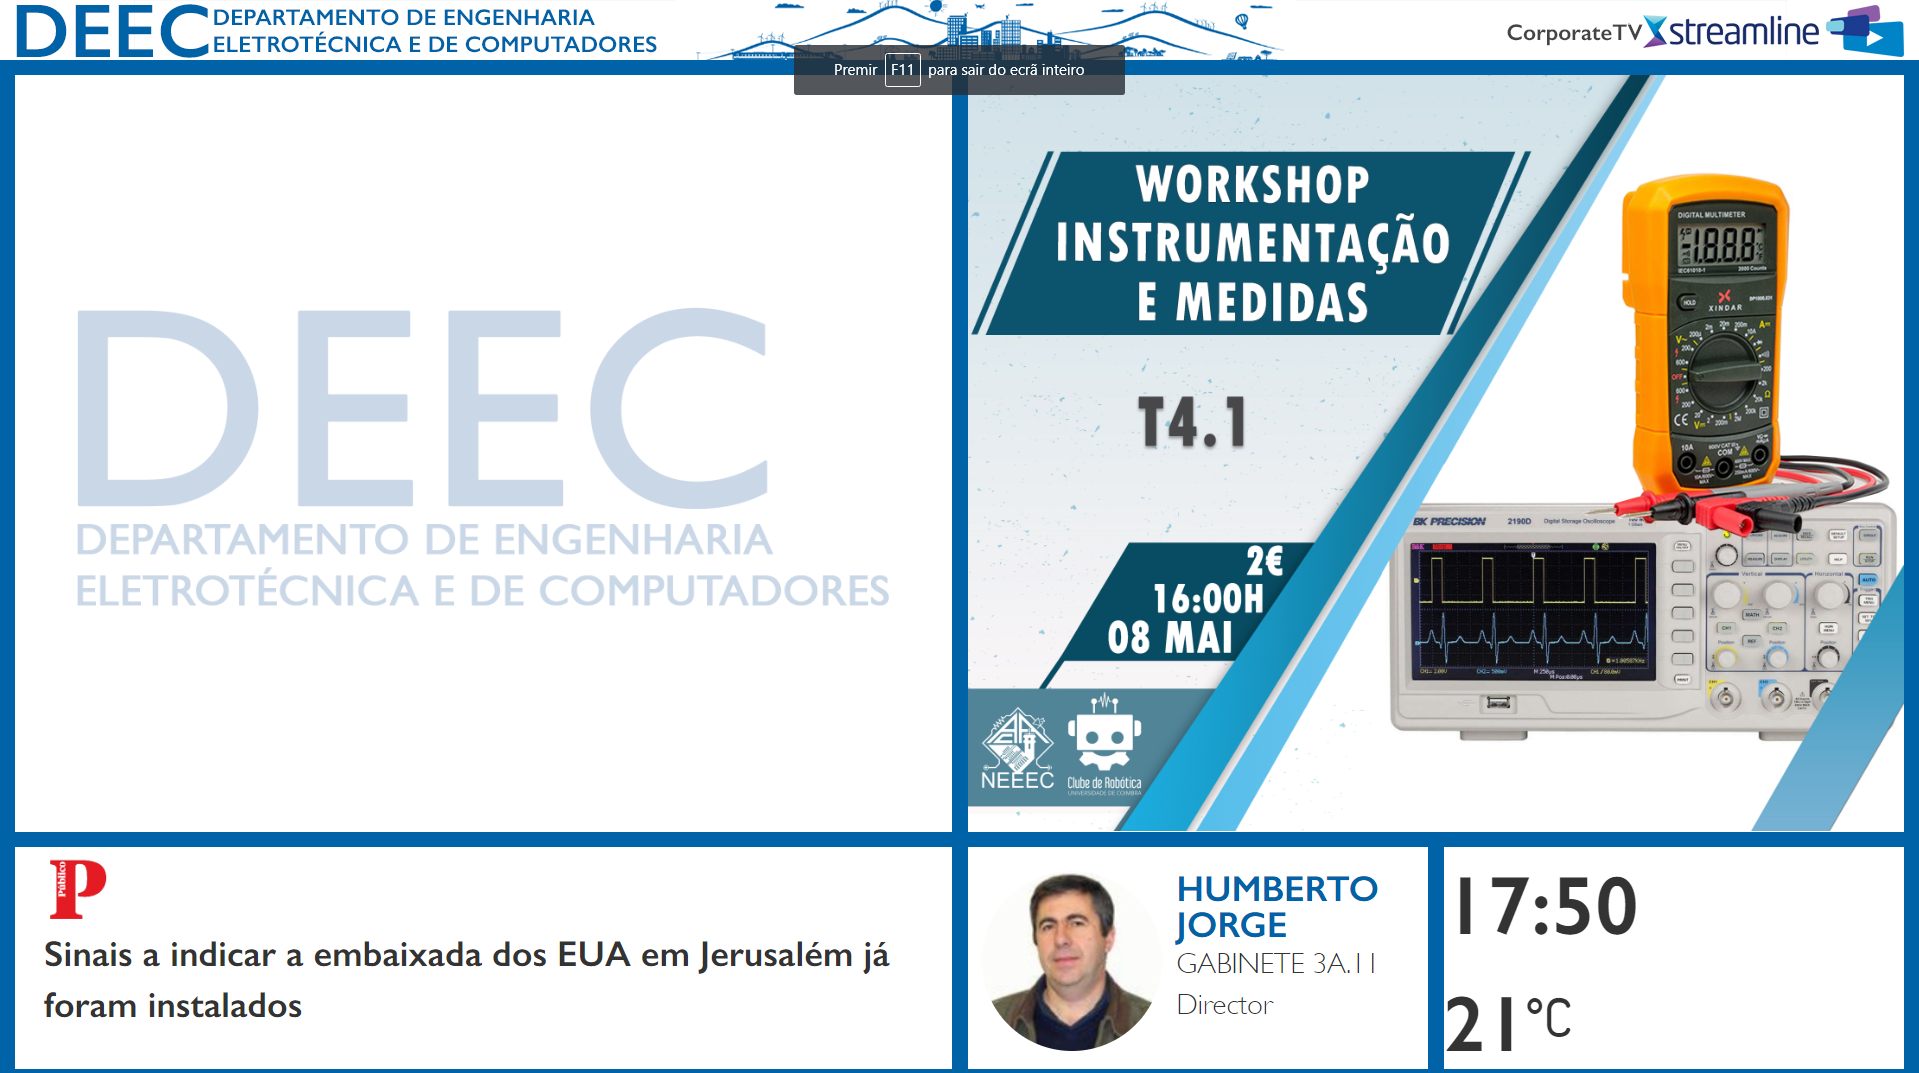
\includegraphics[width=\textwidth]{imagens/tvDEEC1.png}
\caption{Layout antigo.}
\label{fig:tvDEEC1}
\end{figure}

Adicionalmente, após umas obras de remodelação da sala de reuniões do \acrshort{deec}, o professor Humberto Jorge ofereceu uma televisão ao \acrshort{neeec}. Esta televisão foi instalada na sala de convívio tendo também sido instalado um pc que permite a exibição do layout das tv’s do \acrshort{deec} nesse ecrã. O GRI, gentilmente, criou um novo layout específico para o \acrshort{neeec} que ficou em exibição nessa televisão e pode ser visto na figure \ref{fig:tvDEEC2}.

\begin{figure}[ht]
\centering
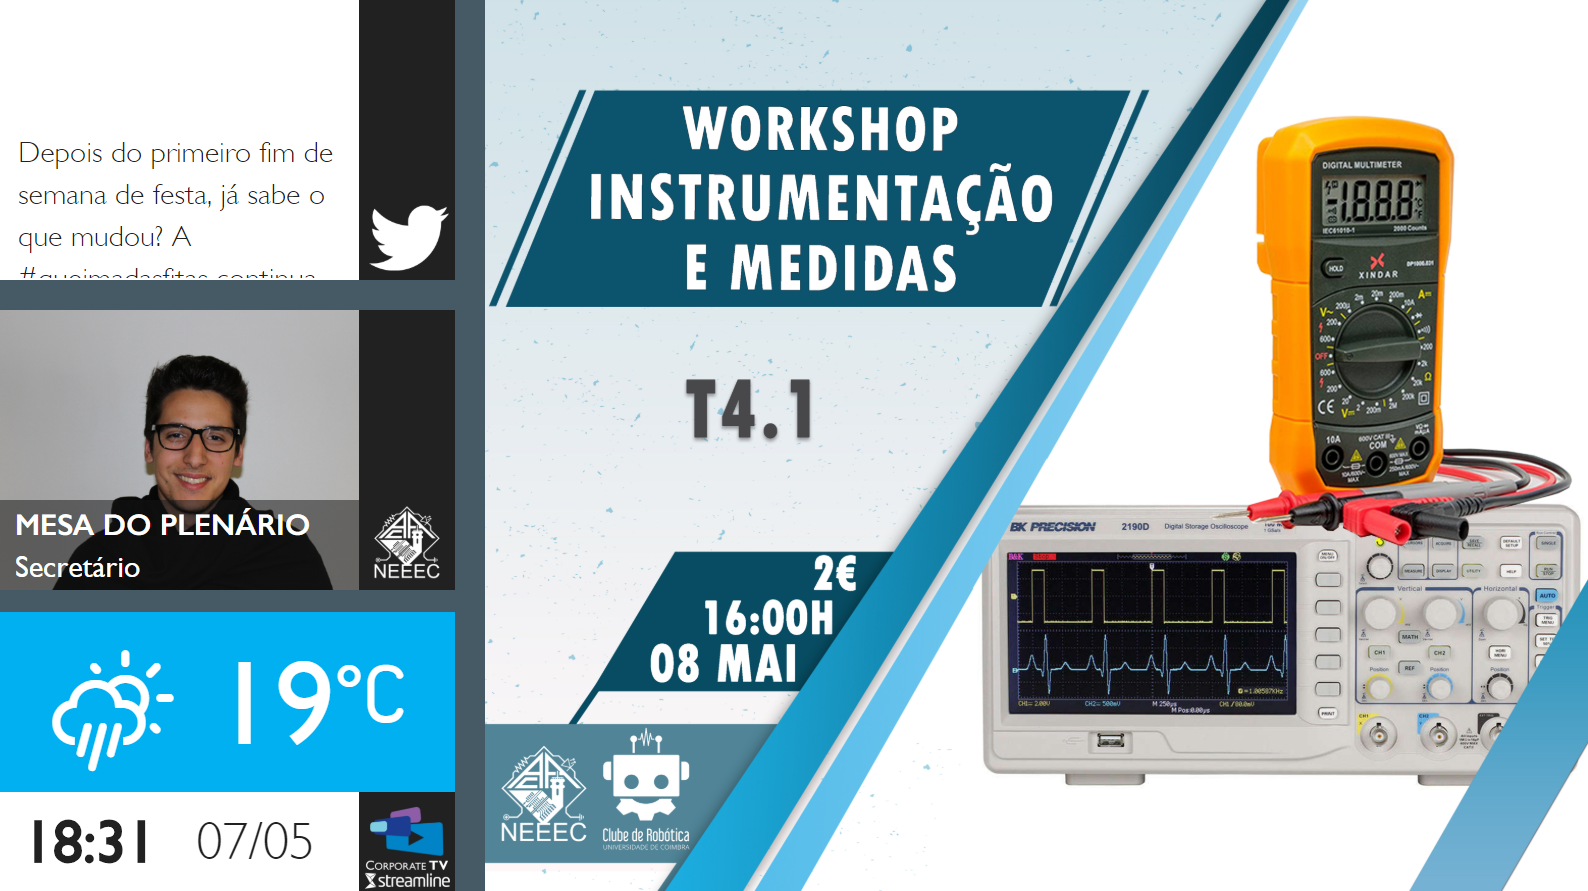
\includegraphics[width=\textwidth]{imagens/tvDEEC2.png}
\caption{Layout criado para o \acrshort{neeec}.}
\label{fig:tvDEEC2}
\end{figure}

Todos os layouts são totalmente configuráveis na plataforma onde se inserem as imagens. As fotos, nomes e cargos dos membros do \acrshort{neeec} que aparecem na tv, podem ser alterados através de um ficheiro que se encontra no servidor onde está alojado o site do \acrshort{neeec}.

\begin{itemize}
\item Inserir imagens/notícias na plataforma:
	\begin{itemize}
	\item Aceder a http://cptv.streamline.pt/\#/login;
    \item Selecionar o ícone de editar ao lado de \acrshort{fctuc} | Departamento de Eng. Eletrónica e de Computadores;
    \item Descer até à secção de imagens e clicar em “Upload de imagens”;
    \item Escolher o(s) ficheiro(s) a enviar;
    \item Ir à galeria de imagens, selecionar a foto que se pretende colocar na notícia e pressionar em “Copiar URL”;
    \item Selecionar “Voltar à edição” e ir à área de notícias, selecionando o ícone do balão de fala para adicionar uma nova notícia;
    \item Caso se pretenda inserir apenas uma imagem, selecionar, no tipo, “Imagem” e colar o URL da imagem no campo devido. Colocar um título na notícia (não irá ser mostrado);
    \item Escolher a data (após a data selecionada como data de fim a notícia irá deixar de estar visível nas televisões);
    \item Carregar em alterar;
    \item Para inserir uma notícia de texto basta, no tipo, selecionar “Informação”. Neste modo é também possível inserir imagens devendo-se proceder da mesma forma para copiar o URL da imagem. Deve-se depois, no campo “Conteúdo”, selecionar o ícone de imagem e colocar a foto que se pretende, dimensionando também o tamanho e escolhendo a posição da imagem no ecrã.
	\end{itemize}
\end{itemize}

Este meio veio facilitar o nosso trabalho por permite a inserção de textos, vídeos e imagens com uma data de início e uma data de fim de divulgação que poderá ser posterior à atual. Desta forma, a imagem ao criar a imagem dos eventos enviava sempre uma imagem para o formato da tv sendo assim possível inseri-la no sistema e ter mais um meio de divulgação que funciona bastante bem, de forma fácil, uma vez que é tem uma divulgação dinâmica e está sempre organizado de forma automática.

% ==========================
% # Notas de Imprensa      #
% ==========================

\paragraph{Notas de Imprensa}

Ao longo do ano existem várias atividades que poderão ser divulgadas facilmente através da imprensa, nomeadamente a regional. Desta forma, achamos que deveria existir alguém no Núcleo designado para ser assessor de imprensa, contudo, novamente pelos problemas referidos sobre o Pelouro das Relações Externas e Comunicação, tal nunca foi feito. Ao longo deste ano, esta tarefa foi feito essencialmente pela Presidência e pelo André Duarte, no caso do Bot Olympics.

Para uma melhor divulgação das notícias é possível entrar em contacto com a assessoria de imprensa da \acrshort{uc}, atualmente gerida pela Dr.ª Cristina Pinto, que facilmente ajuda o \acrshort{neeec} na divulgação de todas as notícias. Foi também possível entrar em contacto com a \acrfull{ruc} e o Jornal "A Cabra", através dos formulários disponíveis nos seus sites, bem como com o "Notícias de Coimbra"\space através do email fernandomoura@noticiasdecoimbra.pt. Ao longo do ano foram sendo sempre criadas \textit{press releases} (como aconteceu na \acrshort{f3e}, no \acrshort{ene3} e no aniversário do Núcleo, por exemplo) que eram divulgados junto das entidades. Mais tarde, os jornais interessados ou vinham ao \acrshort{deec} fazer entrevistas presenciais ou faziam-nas por via telefónica.

% ==========================
% # Ligação C&I e Pelouros #
% ==========================

\paragraph{Ligação C\&I e Pelouros}

A ligação entre a imagem, a comunicação e os diversos pelouros e comissões organizadoras do \acrshort{neeec} foi um dos nossos maiores desafios. Para tal foram criadas várias soluções para este problema:
\begin{itemize}
\item Foi criado um formulário de pedidos de imagem que os Coordenadores deveriam preencher quando querem pedir algo à imagem. Este formulário, uma vez que tinha várias perguntas diretas, fazia com que não fossem esquecidos pormenores importantes que é normal serem esquecidos como, por exemplo, quais as entidades que colaboram com o \acrshort{neeec} nessa atividade e devem aparecer no cartaz.
\item Sala feedback divulgação no Slack: esta era uma sala onde estavam presentes todos os membros da imagem, da comunicação e os CGs dos diversos pelouros sendo o local onde a imagem enviava as versões finais provisórias dos seus trabalhos. Desta forma, todos poderiam corrigir algum erro e opinar sobre a qualidade das imagens, algo que foi muito positivo para a emissão do material a divulgar em concordância entre todos os envolvidos.
\end{itemize}